% Document setup
\documentclass[11pt]{book}

% Location of the csas-style repository: adjust path as needed
\newcommand{\locRepo}{csas-style}

% Use the style file in the csas-style repository (sr.sty)
\usepackage{\locRepo/sr}

% header-includes from R markdown entry
\usepackage{pdflscape}
\newcommand{\blandscape}{\begin{landscape}}
\newcommand{\elandscape}{\end{landscape}}
\newcommand{\beginAppA}{ \setcounter{table}{0}\renewcommand{\thetable}{A\arabic{table}}\setcounter{figure}{0}\renewcommand{\thefigure}{A\arabic{figure}} }

%%%% Commands for title page etc %%%%%

% Title
\newcommand{\rdTitle}{Evaluating the robustness of candidate management procedures in the BC Sablefish (\emph{Anoplopoma fibria}) fishery for 2019-2020}

% French title
\newcommand{\rdTitleFr}{Évaluation de la robustesse des procédures de gestion proposées pour la pêche à la morue charbonnière (\emph{Anoplopoma fimbria}) en C.-B., 2019-2020}

% Title short
\newcommand{\rdTitleShort}{Robustness of Sablefish MPs in BC}
% End of title short

% Publication year
\newcommand{\rdYear}{2020}

% Publication month
\newcommand{\rdMonth}{May}

% Report number
\newcommand{\rdNumber}{\threedigits{025}}
% End of report number

% Approver (name\\position)
\newcommand{\rdApp}{Carmel Lowe\\
Regional Director}

% Approval date
\newcommand{\rdAppDate}{November 4, 2019}

% Branch
\newcommand{\rdBranch}{Science Branch}

% Region
\newcommand{\rdRegion}{Pacific Region}

%%%% End of title page commands %%%%%
% commands and environments needed by pandoc snippets
% extracted from the output of `pandoc -s`
%% Make R markdown code chunks work
\usepackage{array}
\usepackage{amssymb,amsmath}
\usepackage{color}
\usepackage{fancyvrb}
\DefineShortVerb[commandchars=\\\{\}]{\|}
\DefineVerbatimEnvironment{Highlighting}{Verbatim}{commandchars=\\\{\}}
% Add ',fontsize=\small' for more characters per line
\newenvironment{Shaded}{}{}
\newcommand{\KeywordTok}[1]{\textcolor[rgb]{0.00,0.44,0.13}{\textbf{{#1}}}}
\newcommand{\DataTypeTok}[1]{\textcolor[rgb]{0.56,0.13,0.00}{{#1}}}
\newcommand{\DecValTok}[1]{\textcolor[rgb]{0.25,0.63,0.44}{{#1}}}
\newcommand{\BaseNTok}[1]{\textcolor[rgb]{0.25,0.63,0.44}{{#1}}}
\newcommand{\FloatTok}[1]{\textcolor[rgb]{0.25,0.63,0.44}{{#1}}}
\newcommand{\CharTok}[1]{\textcolor[rgb]{0.25,0.44,0.63}{{#1}}}
\newcommand{\StringTok}[1]{\textcolor[rgb]{0.25,0.44,0.63}{{#1}}}
\newcommand{\CommentTok}[1]{\textcolor[rgb]{0.38,0.63,0.69}{\textit{{#1}}}}
\newcommand{\OtherTok}[1]{\textcolor[rgb]{0.00,0.44,0.13}{{#1}}}
\newcommand{\AlertTok}[1]{\textcolor[rgb]{1.00,0.00,0.00}{\textbf{{#1}}}}
\newcommand{\FunctionTok}[1]{\textcolor[rgb]{0.02,0.16,0.49}{{#1}}}
\newcommand{\RegionMarkerTok}[1]{{#1}}
\newcommand{\ErrorTok}[1]{\textcolor[rgb]{1.00,0.00,0.00}{\textbf{{#1}}}}
\newcommand{\NormalTok}[1]{{#1}}
\newcommand{\OperatorTok}[1]{\textcolor[rgb]{0.00,0.44,0.13}{\textbf{{#1}}}}
\newcommand{\BuiltInTok}[1]{\textcolor[rgb]{0.00,0.44,0.13}{\textbf{{#1}}}}
\newcommand{\ControlFlowTok}[1]{\textcolor[rgb]{0.00,0.44,0.13}{\textbf{{#1}}}}

%Defines cslreferences environment
%Required by pandoc 2.8
%Copied from https://github.com/rstudio/rmarkdown/issues/1649

\DeclareGraphicsExtensions{.png,.pdf}
\begin{document}

\bookmark[dest=PageOne]{\rdTitle{}}

\MakeFirstPage

\hypertarget{context}{%
\section{Context}\label{context}}

Since 2008, Fisheries and Oceans Canada (DFO) and the British Columbia (BC) groundfish fishing industry have collaborated on a management strategy evaluation (MSE) process intended to maintain a transparent and sustainable harvest strategy for Sablefish fisheries in BC. Transparency and potential sustainability of candidate management procedures (MPs) are demonstrated by simulating MP performance against a set of pre-agreed biological and fishery objectives (hereafter referred to as Fishery Objectives). Operating models underlying the simulations are intended to represent key uncertainties related to Sablefish stock status and productivity. The Sablefish MSE process has been reviewed in several Canadian Science Advisory Secretariat (CSAS) peer-review processes, and independent peer-reviewed scientific literature (Cox and Kronlund \protect\hyperlink{ref-cox2008practical}{2008}; Cox et al. \protect\hyperlink{ref-cox2011management}{2011}, \protect\hyperlink{ref-cox2013roles}{2013}, \protect\hyperlink{ref-cox2019evaluating}{2019}; DFO \protect\hyperlink{ref-dfo2014performanc}{2014}). Canadian Sablefish harvest advice derived from simulation-tested MPs has been adopted by DFO every year since 2011.

The Sablefish MSE aims to follow a 3-year cycle in which the operating model (OM) is re-fitted to updated fishery and survey biomass indices, catch-at-age, at-sea releases, and tag release-recoveries. Each 3-year update also offers an opportunity to revise the Fishery Objectives, as well as to propose new candidate MPs.

Previous BC Sablefish assessments and MSE work have demonstrated that low recruitment (on average) over the past three decades has contributed to a long-term decline in spawning stock biomass and harvest opportunities. Stakeholder and management consultations identified at-sea release mortality of sub-legal Sablefish (i.e., fish smaller than 55 cm size limit) as a potential source of mortality that, if reduced or avoided, may improve production of over-55 cm Sablefish, spawning stock biomass, and, ultimately, future harvest opportunities (Cox et al. \protect\hyperlink{ref-cox2019evaluating}{2019}). While some voluntary tactics aimed at reducing sub-legal mortality have been identified (e.g., improved fleet communication, and increased electronic monitoring), management measured aimed at reducing sub-legal mortality have not been formally evaluated through the Sablefish MSE process. However, past closed-loop simulations suggest that both full avoidance and full retention of sub-legal Sablefish may improve both average annual Sablefish yield in directed fisheries as well as the probability of stock rebuilding to \(B_{MSY}\) (Cox et al. \protect\hyperlink{ref-cox2011management}{2011}, \protect\hyperlink{ref-cox2019evaluating}{2019}). Unfortunately, full avoidance may not be feasible, especially in trawl fisheries, which encounter sub-legal Sablefish as part of fishing operations for other species, while full retention may involve lost fishing opportunities (particularly for the trawl sector) and lower profitability for directed fisheries, because sub-legal Sablefish are worth less per-kilogram than legal-sized fish. In consultations, industry stakeholders suggested that a potential solution would involve incentives that shift fishing behaviour

toward higher avoidance of sub-legal Sablefish.

The DFO Fisheries Management Branch has, therefore, requested that the Science Branch (i) update the Sablefish OM to include the most recent data available (up to 2018); (ii) update advice about expected performance of the current MP; and (iii) evaluate alternative MP and/or management measures aimed at reducing productivity losses to sub-legal mortality. The key issue in (iii) is identifying MPs that minimize the impact of such measures on fishing opportunities in non-directed fisheries (i.e., trawl) where sub-legal Sablefish are captured incidentally.

Advice arising from this CSAS Science Response will be used to select a new MP for BC Sablefish for years 2020-2022 that is compliant with the DFO Sustainable Fisheries Framework and A Fishery Decision-making Framework Incorporating the Precautionary Approach policy (DFO \protect\hyperlink{ref-DFO2009}{2009}). In addition, this Science Response informs fishery managers and stakeholders about the fishery implications of limiting productivity losses due to sub-legal Sablefish releases at-sea.

This Science Response Report results from the Science Response Process of September 2019 on evaluating the robustness of candidate management procedures in the BC Sablefish (\emph{Anoplopoma fibria}) fishery for 2019-2020.

\hypertarget{analysis-and-response}{%
\section{Analysis and response}\label{analysis-and-response}}

This Science Response uses a closed-loop simulation approach to evaluate the relative performance of candidate MPs for the BC Sablefish fishery, using identical methodology to that presented in the previous MSE cycle (Cox et al. \protect\hyperlink{ref-cox2019evaluating}{2019}). The following sub-sections provide brief descriptions of the updated data used to condition the Sablefish OM, the changes required to fit that data, and the new MP elements that were tested. Additional details of the simulation procedures, diagnostic checks, and performance measure calculations are given in Cox et al. (\protect\hyperlink{ref-cox2019evaluating}{2019}).

In this Science Response we specifically:
\begin{enumerate}
\def\labelenumi{\arabic{enumi}.}

\item
  Describe OM fits and inferences after fitting (conditioning) to updated biomass indices, catch-at-age, and new catch-at-age data derived from length-composition sampling of Sablefish in the trawl fishery;
\item
  Derive a grid of five reference OMs and five robustness trial OMs based on uncertainties about Sablefish stock status and productivity (reference OMs) and year 2015 recruitment (robustness OMs); and
\item
  Simulate and rank candidate MPs under the reference and robustness OMs based on performance against Fishery Objectives (see below).
\end{enumerate}
\hypertarget{methods}{%
\subsection{Methods}\label{methods}}

\hypertarget{updates-to-the-om}{%
\subsubsection{Updates to the OM}\label{updates-to-the-om}}

Data updated to 2018 included biomass indices and catch-at-age for the stratifed random trap survey (StRS), catch-at-age for the commercial longline trap fishery, catch and total at-sea releases (in biomass units) for the commercial longline trap, longline hook, and trawl fisheries. We also obtained new catch-at-age and catch-at-length datasets for the trawl fishery to help estimate trawl selectivity, which is the key determinant of sub-legal Sablefish catch in trawl fisheries. The full trawl catch-at-age dataset (with some missing years) was derived from an age-length key given age and length data from 1972 to 2017.

A number of small changes were made to the OM as part of routine attempts to improve fits to various data. These included (i) changing the functional form of trawl selectivity to a gamma density function (Figure A5), (ii) reducing the youngest modelled age class from age-3 to age-2 for all age composition series to better reflect the range of age-composition observations, (iii) adding new commercial trawl age-composition data (Appendix A), (iv) adding an estimated recruitment deviation in 2015, rather than using the expected recruitment off the stock-recruit curve, (v) updating the ageing-error matrix to use a simpler normal approximation recommended in the previous CSAS review (Cox et al. \protect\hyperlink{ref-cox2019evaluating}{2019}); and (vi) imposing a standard deviation of \(\sigma = 0.1\) (on the log-scale) on trawl at-sea release observation errors to force a better fit to those data. Previous models avoided estimating recruitment in the three most recent years, mainly because this would have been the first age-at-entry observations provided to the model and there is typically little information to support those estimates because fish are too small to be selected by the fisheries or surveys. However, for this update, we made change (iv) above (i.e., estimated recruitment deviation in 2015) because we needed to improve fits to recent (very high) trawl at-sea release observations. Otherwise, we would be simulating effects of at-sea releases based on a model that could not adequately fit historical at-sea releases. This change has a potentially large impact on simulated MP performance and, therefore, is a focus of the robustness OMs (described below).

\hypertarget{operating-model-scenarios}{%
\subsubsection{Operating model scenarios}\label{operating-model-scenarios}}

Reference OMs were derived using the same method as the previous MSE cycle (Cox et al. \protect\hyperlink{ref-cox2019evaluating}{2019}). Briefly, we derived five OMs defined by the joint posterior distribution of 2018 spawning stock biomass (to reflect short-term biological risk) and stock-recruitment steepness (to reflect long-term stock productivity risk). The five combinations were chosen to represent the joint marginal mean of 2018 biomass and steepness and four outer points lying at the intersection of the mean of one variable, and the 10th and 90th percentiles of the marginal density of the other variable (Figure 1). This set of five OMs was chosen to maintain consistency with the previous MSE cycle (Cox et al. \protect\hyperlink{ref-cox2019evaluating}{2019}). For each of the five posterior points, the operating model was conditioned on a sample of 100 posterior draws constrained to lie within a Mahalanobis distance of 0.75 units from that point. We then used an empirical estimate of the posterior density at each of the five centres as a plausibility score for weighting MP performance across the five OMs within each of the reference and robustness sets.

Robustness OMs were identical to the five reference OMs with the exception of how the recruitment from the 2015 year class was treated in the OM historical conditioning and projections. The reference OM used draws from the joint posterior distribution (as defined above) for the 2015 year class, which is approximately 22 million fish or about 8 times the historical average. For the robustness OMs, we simulated recruitment based on the stock-recruitment relationship resulting in an expected 2015 year class that was more similar to the long-term average (\(\sim 2.63\) million).

\hypertarget{fishery-objectives}{%
\subsubsection{Fishery Objectives}\label{fishery-objectives}}

Objectives for the B.C. Sablefish fishery have been developed iteratively over the past decade via consultations between fishery managers, scientists, and industry stakeholders (Cox and Kronlund \protect\hyperlink{ref-cox2009evaluation}{2009}; Cox et al. \protect\hyperlink{ref-cox2011management}{2011}, \protect\hyperlink{ref-cox2019evaluating}{2019}; DFO \protect\hyperlink{ref-dfo2014performanc}{2014}). The five primary objectives guiding this fishery are:
\begin{enumerate}
\def\labelenumi{\arabic{enumi}.}

\item
  \textbf{P(fSSB \textgreater{} LRP)}: Maintain female spawning stock biomass (fSSB) above the limit reference point \(LRP = 0.4B_{MSY}\), where \(B_{MSY}\) is the OM female spawning biomass at maximum sustainable yield (\(MSY\)), in 95\% of years measured over two Sablefish generations (36 years);
\item
  \textbf{P(decline)}: When female spawning stock biomass is between \(0.4B_{MSY}\) and \(0.8B_{MSY}\), limit the probability of decline over the next 10 years from very low (5\%) at \(0.4B_{MSY}\) to moderate (50\%) at \(0.8B_{MSY}\). At intermediate stock status levels, define the tolerance for decline by linearly interpolating between these probabilities;
\item
  \textbf{P(fSSB \textgreater{} \(B_{MSY}\))}: Maintain the female spawning biomass above a target level of (a) \(B_{MSY}\) when inside the healthy zone, or (b) \(0.8B_{MSY}\) when rebuilding from the Cautious zone, in the year 2052 with a probability of 50\%;
\item
  \textbf{P(TAC \textless{} 1,992 t)}: Minimize probability that annual TAC levels are below 1,992 tonnes measured over two Sablefish generations; and
\item
  \textbf{MaxCatch}: Maximize the average annual catch over 10 years subject to Objectives 1-4.
\end{enumerate}
Performance measures corresponding to Fishery Objectives 1-4 (in bold) are read as ``Probability of (condition)''. Performance measures are calculated for each simulation replicate, and the expected performance for a management procedure is summarized by the mean (or median) over the 100 replicates of each simulation. Full details of performance measures and calculations are given in Cox et al. (\protect\hyperlink{ref-cox2019evaluating}{2019}).

As noted above, there is a price premium for larger size classes of Sablefish, which means that the same tonnage of landed catch may yield widely different dockside values if the underlying size distributions of individual fish are substantially different. This may have consequences for sub-legal management measures that require landing small Sablefish (e.g., no size limit). Therefore, in addition to presenting catch performance statistics (e.g., Fishery Objective 5), we also computed cumulative revenue over 10 years and average revenue per tonne by fleet (because the size composition of the catch also differs by fleet).

\hypertarget{management-procedures}{%
\subsubsection{Management procedures}\label{management-procedures}}

A management procedure represents a specific, repeatable algorithm for computing annual total allowable catches (TACs) in a fishery. In most cases, MPs involve monitoring data, assessment methods for processing data and estimating stock status, harvest control rules for translating assessment outputs into catch limits, and meta rules that may include constraints on TAC changes, as well as conditions (e.g., exceptional circumstances) for triggering deviations from the standard MP harvest advice.

The MP currently used to set annual Sablefish TACs was initially developed in 2011 and revised in two subsequent MSE iterations. Generally, the MP consists of (i) \textbf{data} - landed catch and three biomass indices; (ii) \textbf{assessment method} - a surplus production model with observation and process errors for estimating stock biomass from the biomass indices and landings; (iii) \textbf{harvest control rule} - a 60:40 harvest control rule (HCR) in which the target harvest rate is adjusted from 0\% when the estimated biomass is below 40\% of \(B_{MSY}\) to a maximum value when estimated biomass is above 60\% of estimated \(B_{MSY}\); (iv) \textbf{a meta rule} stating that TAC increases are 0 unless the HCR recommended increase is more than 200 tonnes (TAC decreases are always adopted); and (v) \textbf{a meta rule} adjusting the maximum target fishing mortality rate from 9.5\% in 2017 to 5.5\% in 2021. Total TACs are allocated among the three sectors according to 40.37\% for longline trap, 50.90\% for longline hook, and 8.75\% for trawl, with the remaining quota being reserved for surveys. The trawl allocation is based on negotiations between the sectors that fixed trawl allocation in previous MSE work (Cox et al. \protect\hyperlink{ref-cox2011management}{2011}), while the trap and hook split is calculated based on the average proportion of catch in each sector over the years 2009 - 2018.

For this Science Response, we evaluated performance of the current MP for Sablefish, a no fishing reference case, and 15 variations of the current MP that only vary in their at-sea release management measures. The MP variants are constructed by combining three features:
\begin{enumerate}
\def\labelenumi{\arabic{enumi}.}

\item
  \textbf{at-sea sub-legal release cap} in which all at-sea releases below the cap may be released without penalty and amounts exceeding the cap go to overages. Caps are noCap, 0\%, 50\%, 100\%, and 150\% over the average 464 t of at-sea releases that occurred between 2006 and 2018. The current MP involves no cap (unlimited at-sea releases without penalty), while a no size limit (\textbf{NSL}) case allows no at-sea releases (all fish brought on-board vessels must be landed and counted against the TAC).
\item
  \textbf{fixed allocation among fleets} (i.e.~trap, longline hook, trawl) of the total at-sea release cap. Allocations are computed based on either recent (rct = \((23\%, 18\%, 59\%)\), 2016 - 2018) or historical (hst = \((30\%, 37\%, 33\%)\), 2006-2018) fleet-specific average proportions of the total annual at-sea releases.
\item
  \textbf{amortization period} of either 5 (am5) or 10 (am10) years over which to spread at-sea release overages to future TACs.
\end{enumerate}
In this Science Response, MPs are named by combining the three at-sea management measures detailed above: CAP\_ALLOCATION\_AMORTIZATION. For example, the \textbf{cap.5\_hstAl\_am5} MP involves a total at-sea release cap that is 50\% (0.5) of the historical average (\textbf{cap.5}), a cap allocation among fleets that is based on the historic (2006-2018), fleet-specific average proportions (\textbf{hstAl}), and a 5-year amortization period for at-sea release overages (\textbf{am5}). The two special cases to this naming convention are the current MP (\textbf{noCap}), which has no cap, and no size limit MP (\textbf{NSL}), which has no releases (all fish are landed, regardless of size). For 0\% caps, only the amortization period for overages would apply (e.g. \textbf{cap0\_am5}) with all at-sea releases counted as overages.

\hypertarget{a-worked-example-at-sea-release-management-measures-for-cap.5_hstal_am5.}{%
\subsubsection{\texorpdfstring{A worked example at-sea release management measures for \textbf{cap.5\_hstAl\_am5}.}{A worked example at-sea release management measures for cap.5\_hstAl\_am5.}}\label{a-worked-example-at-sea-release-management-measures-for-cap.5_hstal_am5.}}

To illustrate how we simulated the implementation of the at-sea release management measures, below we provide the sequence of calculations used to establish annual at-sea release caps and then how they affect future TAC allocations. In the computations below, \(t\) is year, \(g\) is fleet, and \(p(g)\) is proportion of releases allocated to fleet \(g\).
\begin{enumerate}
\def\labelenumi{\arabic{enumi}.}

\item
  Calculate 50\% at-sea release CAP for year and fleet (464 t is the 2006 - 2018 average): \begin{equation*}
        CAP(t,g) = 0.5 \cdot 0.464 \cdot p(g).
  \end{equation*}
\item
  Run simulation for year t to get actual at-sea releases: \(R(t,g)\).
\item
  Calculate overage \(o(t,g)\) for the year as the difference between actual releases \(R(t,g)\) and the \(CAP(t,g)\): \tabularnewline \begin{equation*}
        o(t,g) = R(t,g) - CAP(t,g).
  \end{equation*}
\item
  Amortization period is 5 years, so add 1/5th of this year's overage. to the accumulated overage account \(O(t+k,g)\) in each of the next 5 years: \begin{equation*}
        O(t + k,g) = O(t+k,g) + o(t,g)/5, \mbox{ for } k = 1, ..., 5.
  \end{equation*}
\item
  Get adjusted legal-sized Sablefish TAC for next year by subtracting overage account for that year from initial \(TAC'\) (\(TAC'\) set by the MP prior to at-sea management measures): \begin{equation*}
        TAC(t,g) = TAC'(t,g) - O(t,g).
  \end{equation*}
\end{enumerate}
This approach aims to create an incentive to avoid sub-legal Sablefish via future TAC reductions (assuming one-for-one accounting of sub-legal biomass to legal sized Sablefish biomass), while also allowing some flexibility year-to-year for unpredictably large at-sea releases in any given year. Note that the overage account can never be less than zero, so that TACs cannot be increased above the initial TAC set by the first stage MP (i.e., banking of TAC cannot occur).

\hypertarget{management-procedure-tuning}{%
\subsubsection{Management procedure tuning}\label{management-procedure-tuning}}

The Sablefish management strategy evaluation quantifies MP performance against performance statistics representing each of the the Fishery Objectives. The first three performance statistics are represented by biomass conservation performance against the LRP, short-term probability of decline, and achieving a long-term target at or near \(B_{MSY}\), while the fourth and fifth ones relate to maintaining catch levels above an industry-preferred floor and short-term average catch. It is rare that two MPs would have comparable performance across four of these performance statistics while only differing on one. If this were the case, then the decision on which MP is preferred would be straightforward -- choose the MP with better performance on the fifth statistic. Unfortunately, MPs typically differ on all five performance statistics simultaneously, which makes it difficult to compare performance without, at least, establishing some equivalency between conservation probabilities (Fishery Objectives 1-3) and short-term average catch (Fishery Objectives 5).

Management procedure tuning provides a means of establishing equivalent MP performance against objectives for which the values and probabilities are well established. For example, maintaining the Sablefish stock above the LRP (\(0.4B_{MSY}\)) with high probability has not been openly debated since it is an overarching Canadian policy directive in the Sablefish fishery context (at least not debated over the 10+ year history of the Sablefish MSE). Similarly, maintaining a low probability of short-term decline has also not been debated, probably because avoiding further decline has been the key overriding objective of the Sablefish fishing industry since the inception of the MSE process. Fishery Objective 3 -- spawning biomass in the healthy zone within 2 generations -- has been debated over the years for practical reasons. Specifically, there is concern that achieving Fishery Objective 3 would require severe short-term catch restrictions for highly uncertain long-term benefits. Over the past year, the Sablefish industry and DFO agreed to revise Fishery Objective 3 to achieve biomass in the healthy zone by a specific end-year (2052) with at least 50\% probability, i.e., median fSSB at, or above, \(B_{MSY}\). As we demonstrate below, this objective is now feasible given Sablefish dynamics and also achievable for a range of realistic MPs. However, this raises a new question: how much is it worth (i.e., in catch) to improve Fishery Objective 3 performance from, say, \(P(B_{2052} \geq B_{MSY}) = 0.5\) to \(P(B_{2052} \geq B_{MSY}) = 0.55\)? The probability difference of only five percentage points could mean a difference of several hundred tonnes in average annual catch, which would cumulatively add up to tens of millions of dollars in revenue. MPs that perform better under Fishery Objective 3 almost always do so at the expense of performance under Fishery Objectives 4 and 5.

We aimed to simplify interpretation of MP performance by tuning all MPs to a standard \(P(B_{2052} \geq B_{MSY}) = 0.5\), which ensured that all MPs meet Fishery Objectives 1-3.Tuning was achieved by iteratively adjusting \(F_{2021}\), which is the maximum target fishing mortality rate scheduled for Year 2021 (as part of 5-year phase-in period for the current MP) (Cox et al. \protect\hyperlink{ref-cox2019evaluating}{2019}), until each MP satisfied Objective 3, i.e., \(P(B_{2052} \geq B_{MSY}) = 0.5\). These \(F_{2021}\) target maximum harvest rates then replace the scheduled maximum target harvest rate of 5.5\% for Year 2022 and beyond.

Each MP was tuned seperately to the reference and robustness OM scenarios, leading to different \(F_{2021}\) values for each MP (i.e., once for each OM). We then simulated a cross-test in which \(F_{2021}\) values tuned under the reference OM were applied in MPs for the robustness OM and vice versa. The cross-test reveals the potential biological and catch consequences of using the wrong \(F_{2021}\) values.

\hypertarget{results}{%
\subsection{Results}\label{results}}

\hypertarget{operating-model-update-and-implications-for-stocks-status}{%
\subsubsection{Operating model update and implications for stocks status}\label{operating-model-update-and-implications-for-stocks-status}}

Operating model fits to survey and fishery biomass indices were similar to previous versions, where both the model and data showed a long-term steady decline. The most recent two stratified random survey (StRS) data points (2017 and 2018) were substantially higher than the preceding 15 years, suggesting potential increases in the offshore stock biomass (Figure 2).

In general, the age-structured OM fit the age-composition data reasonably well (Figure 3). Fits to the trap fishery age-composition continued to show a large positive residual at the plus-group age 35+ for males, and to a more neglibale extent for females (Figure 3, Trap:). Fits to the trawl age-composition also also showed a large positive residual for age-2 males, which appeared to arise from the 2017 and 2018 samples that were large and, therefore, tended to drive the average to have what appeared to be a large positive residual at age-2. This was a potential contributing factor to the estimated size the estimated 2015 year-class.

Model fits to the standardized survey were similar to previous OM versions --- patterns lie somewhere between the fishery age-composition fits (worst) and StRS fits (best) (Figures 2 and 3). The OM continued to fit StRS very well, which probably arose because the StRS is specifically designed for monitoring the offshore Sablefish population (unlike all other data series).

The updated stock status of Canadian Sablefish depended on the absolute size of the 2015 year-class (age-3 in assessment Year 2018). The raw estimate of this year-class was about eight times the historical average (see Robustness OMs section above; Figure 4, bottom row), which created the impression of the largest recorded recruitment from one of the lowest spawning biomasses ever observed. Such a high recruitment at low spawning biomass had cascading effects on the model parameter estimates, biological reference points, and estimated current biomass. These effects included: (i) the estimated stock productivity (i.e., stock-recruitment steepness parameter) was adjusted upwards; (ii) the most productive stock size (\(B_{MSY}\)) was adjusted downwards, because the stock is apparently more productive at low biomass; (iii) the optimal fishing mortality rate (\(F_{MSY}\)) was adjusted upwards because the more productive stock can sustain higher fishing pressure; and (iv) current spawning biomass was adjusted upwards because about 20-25\% of age-3 fish were maturing. Although these were positive and encouraging signs that Sablefish status is improving, there was some risk in tuning future MPs to substantial model changes that arose from a small number of observations. Other Pacific groundfish fisheries (e.g., Pacific Hake {[}\emph{Merluccius productus}{]} and Gulf of Alaska Sablefish) have treated initial large estimated recruitments with caution until the data used to estimate them more fully materialize. Here, we dealt with the uncertainty in 2015 year-class size by developing reference (using age-3 data) and robustness (ignoring age-3 data) OMs for use in evaluating MPs.

Under the large 2015 year class, the OM fit showed the Sablefish stock status as generally good (Table 1, 2018 Fit). Spawning biomass in 2018 was about twice the limit reference point (LRP), up from about 1.5 times the LRP, which was itself revised from the 2016 fit of about 1.17 times the LRP . This change indicated that the BC Sablefish stock might have moved out of an overfished state. Similarly, the posterior probability of the last year's biomass being above the limit reference also improved from 2016 to 2018, increasing from 93\% (2016 fit) to 100\% (2018 fit).

\hypertarget{management-procedure-evaluation-results}{%
\subsubsection{Management procedure evaluation results}\label{management-procedure-evaluation-results}}

\hypertarget{reference-om-set-under-reference-f_2021-tuning}{%
\subsubsection{\texorpdfstring{Reference OM set under reference \(F_{2021}\) tuning}{Reference OM set under reference F\_\{2021\} tuning}}\label{reference-om-set-under-reference-f_2021-tuning}}

As expected, recruitment from the 2015 year class was the primary driver of projected spawning biomass and fishery outcomes in the reference OM simulations. Spawning biomass increased rapidly over the first five years of the projection period as age-3 (i.e., 2015 year class) fish became fully recruited to the fisheries and then the spawning biomass (Figures 4 and 5, top row). Spawning biomass then trended downward toward \(B_{MSY}\) over the long-term as the 2015 year class was fished down and recruitments returned to expected values around the stock-recruitment relationship (i.e., recruitments for 2016 onward are all simulated off the stock-recruitment relationship).

Under these conditions, all MPs met all the biological criteria defined by Fishery Objectives 1-3 (Table 2). All tuned MPs were able to meet Fishery Objective 3, where median spawning biomass (top row of Figure 5) achieves \(B_{MSY}\) (horizontal dashed line with green dots at end points) by the final year (2052). Some MPs are able to achieve \(B_{MSY}\) 15-20 years prior to the final year, while others just make \(B_{MSY}\) by the final year.

Tuning MPs to meet Fishery Objectives 1-3, and specifically treating Fishery Objective 3 as a target, focuses MP performance differences on average annual catch over the next 10 years (Table 2; Fishery Objective 5). As expected, MPs with more restricted at-sea release management measures ranked higher in terms of 10-year average catch (Table 2) with the values ranging from 4,530 t per year for no size limit (MP17 \textbf{NSL}) to 3,710 t per year for management measures with a cap 150\% higher than average, recent cap allocation among fleets (i.e., allocating 59\% to trawl), and 5-year amortization (MP14 \textbf{cap1.5\_rctAl\_am5}). This difference was attributable to two factors. First, the key assumption here was that fishing activity stops once the TAC is reached, so no size limit results in less mortality of sub-legal fish over all fleets. This led to a large reduction in growth overfishing for the no size limit MP --- gains in Sablefish body growth were much higher than losses due to natural mortality in sub-legal size classes --- and, therefore, average weight of legal-sized fish in the catch is larger. Second, the fishery could operate at higher fishing mortality rates because survival over sub-legal size classes was higher and therefore more fish recruit to fisheries and the spawning stock. Indeed, the apparently conservative current MP maximum target \(F=5.5\%\)/yr was largely the result of lower survival through sub-legal size classes, which inhibited MPs from meeting the future spawning biomass Fishery Objective 3. In contrast, the no size limit MP almost met Fishery Objective 3 despite a maximum target \(F=7.5\%\)/yr on legal-sized fish (Table 2; \(F_{2021}\)).

Differences in average annual catch were smaller among at-sea management measures that involved a size limit. A 0\% at sea-release cap and five year amortization (MP6) resulted in catches about 400 t higher than the current MP (MP15; Table 2), while the gain was 300 t for a 10-year amortization (MP5).

An at-sea release cap of 50\% of the historical average resulted in average annual catch levels 160 t and 300 t higher than the current MP, depending on the allocation and the amortization period (MP3 and MP4 vs.~MP15; Table 2). Interestingly, a 10-year amortization with a 0\% cap gives identical 10-year average catch to a 50\% cap with a historical allocation and 5-year amortization period (MP5 vs MP6; Table 2).

An at-sea release cap equal to 100\% of the historical average also produced 200 t more average annual catch than the current MP, as long as the cap was allocated according to the historical at-sea release proportions and amortized over five years (MP8 vs MP15, Table 2). The similarity to the lower 50\% caps described above mainly reflects cap allocation to the trawl fleet, where the recent allocation (59\%) is approximately twice the historical (33\%), so switching to the lower, historical allocation allowed for doubling the cap, i.e., the total at-sea release amounts allocated to the trawl fleet were similar. In general, the historical allocation options ranked higher than the recent allocations because the historical allocation involves lower at-sea releases by the trawl fleet. The amortization period did not have as noticeable an effect as the overall cap and allocation options, in that order.

Increasing the cap to 150\% of the historical average produced the lowest average annual catch, despite the current MP having no cap at all (MP13 vs 15; Table 2). Although average 10-year catches were similar, at-sea releases in the current MP (\textbf{noCap}) change mainly with recruitment and therefore have less impact than a 150\% cap, which decoupled at-sea releases and recruitment to some (small) degree and allowed trawl fishing to continue past current sub-legal catch rates.

As caps increased under recent at-sea release allocation, the effect of amortization switched from 5 years being better (under low caps) to 10 years being better (under high caps). Although the differences were small (MP12 vs MP3; Table 2), the switch probably occured because there is little to no growth overfishing benefit of amortization at high caps and recent allocations, which would mean higher trawl releases than present. In this case, the amortization period had a direct effect on TACs, with longer amortization periods having less impact because overages spread over the longer period have less impact on annual TAC adjustments.

We initially expected that a no size limit and/or lower cap management measures would negatively affect fishery revenue because the landed catch would consist of higher proportions of sub-legal fish. Price premiums for Sablefish (Table 3; C. Acheson per comm., Spring 2019) may result in several dollars per pound difference between sub-legal (\textless{} 3 lbs) and large (4/5+) legal-sized Sablefish.

Indeed, the average revenue per tonne was approximately \$170 lower for a no size limit trap fishery compared to noCAP (Table 4), while revenue was approximately \$20 and \$1,070 per tonne lower for longline hook and trawl landings, respectively. Size-selectivity for trap, and especially longline hook, fisheries is shifted far enough toward larger sizes that the impacts of retaining smaller fish are relatively small compared to the benefits of higher average TACs. Cumulative revenues over ten years were \$47 million, \$18 million, and \$15 million higher for trap, longline hook, and trawl fisheries under the no size limit MP compared to the next best MP from an average annual catch perspective (i.e., MP6, \textbf{cap0\_am5}; Table 4).

The next best at-sea release management measures, from a total catch and cumulative revenue perspective, after the no size limit MP were different between trap and longline hook fisheries and trawl. For instance, as noted above, MP6 (\textbf{cap0\_am5}) was the next best option for trap and longline hook, in terms of both average annual TAC and cumulative revenue (Table 4). In contrast, the next best option for trawl revenue was MP14 (\textbf{cap1.5\_rctAl\_am5}), which had the lowest average annual TAC. The revenue difference for trawl between this option and no size limit was only \$5 million over 10 years, while the revenue differences between MP6 and MP17 for trap and longline hook were \$33 million and \$32 million, respectively. Thus, the results suggest trap and longline hook fisheries would benefit from more restrictive at-sea management measures while trawl would benefit from the least restrictive at-sea management measures other than the status quo, even without considering the implications for trawl's main target fisheries.

\hypertarget{robustness-om-set-under-robustness-f_2021-tuning}{%
\subsubsection{\texorpdfstring{Robustness OM set under robustness \(F_{2021}\) tuning}{Robustness OM set under robustness F\_\{2021\} tuning}}\label{robustness-om-set-under-robustness-f_2021-tuning}}

Unlike the reference OMs, in which biomass and catch increases were large over the next decade, Sablefish biomass and catch projections under the robustness OMs increased more gradually, and generally required lower fishing rates to meet Fishery Objecitives 1-3 (Figures 6 and 7). In fact, these simulations closely resemble previous Sablefish MSE results, which suggested that relatively conservative harvest strategies are needed over the long-term to meet the Fishery Objecitives 1-3 (Cox et al. \protect\hyperlink{ref-cox2019evaluating}{2019}).

Tuning MPs to meet Fishery Objective 3 under the robustness OMs was more challenging because higher \(F\)s had more noticeable impacts on the short-term decline objective (P(decline); Table 5). MP tuning produced relatively low target fishing mortality rates ranging from 5.2\% (current MP) to 7.2\% (cap0). These low \(F\)s also had the effect of a higher probability of catches less than the 1,992 t (Fishery Objective 4); whereas these were negligible (\textless{} 3\%) in the reference OMs, they were all greater than 15\% in the robustness OMs except under the no size limit MP, which was 8\% (Table 5).

Average annual catch under the robustness OMs ranged from 2,305 t under the current MP (MP15, noCap) to 2,767 t under no size limit (MP17, NSL). Thus, the current MP with no limit on at-sea releases performed worse than any of the cap options by as much as 200 t per year for the top-ranking cap options (Table 5). There was a slight difference in the rank order of MPs (ranked by average 10-year catch) under the robustness OMs compared to the reference OMs, although the absolute difference among most MPs was small.

Average annual variation in catch (AAV) was 9-11\% under the robustness OMs compared to 7-8\% under the reference OMs (Table 5). This probably occurs because the stock remains below \(B_{MSY}\) for most of the projection period and is, therefore, assessed below \(B_{MSY}\) at times. Assessment changes in both stock status and the maximum target fishing mortality have been relatively common in realized applications of Sablefish MPs over the past several years and this causes higher interannual variability in TACs.

Cumulative 10-year revenue under the robustness OMs was approximately 60\% of revenue in the reference OMs (Table 6). Although the absolute scales differ, the cumulative value patterns were similar to the reference set; that is, no size limit produced the highest overall value, as well as value in each fleet, and the next best at-sea release management measure option, from a cumulative revenue perspective, was the most restrictive for trawl and next-most-restrictive for trap and longline hook (MP6, \textbf{cap0\_am5}; Table 6).

\hypertarget{cross-tests-of-oms-under-opposite-f_2021-tuning}{%
\subsubsection{\texorpdfstring{Cross tests of OMs under opposite \(F_{2021}\) tuning}{Cross tests of OMs under opposite F\_\{2021\} tuning}}\label{cross-tests-of-oms-under-opposite-f_2021-tuning}}

As expected, there was considerable asymmetry of risk between MPs tuned under the robustness OMs and reference OMs. For example, when MPs were tuned to meet Fishery Objecitives 1-3 under the reference OMs, but the 2015 year class failed to materialise as in the robustness OMs, almost all MPs failed to meet the performance criteria for Fishery Objectives 2 and 3 (Table 7). The benefit of accepting this conservation risk was approximately 150 t of extra annual catch, or at most a 6\% increase in average annual catch.

On the other hand, if MPs were tuned to meet Fishery Objecitives 1-3 under the robustness OMs, but the 2015 year class materialised as expected under the reference OMs, then, all MPs continued to meet the Fishery Objecitives 1 - 3 (Table 8). This more risk averse strategy (from a biological perspective) comes with the cost of reduced average annual catch of approximately 300 t for all MPs, or 6.5-8\% of the reference-tuned catch.

\hypertarget{conclusions}{%
\section{Conclusions}\label{conclusions}}

The current MP for Canadian Sablefish (MP15, \textbf{noCap}), which includes no limits on at-sea releases, was able to meet biological objectives (i.e., Fishery Objectives 1-3) under both reference and robustness OMs, although it ranked near the bottom in terms of catch performance compared to MPs with at-sea release management measures. Of the MPs with management measures for at-sea releases, MP14 (no size limit), MP17 (0\% cap, 5 year amortization), MP3 (50\% cap, historical allocation, and 5-year amortization) ranked among the top-3 most often under both reference and robustness OMs, provided that maximum target fishing mortality rates were tuned to meet the first three Fishery Objectives.

As indicated in previous MSE work, no size limit MPs result in the highest average annual landed catch while still allowing the fishery to meet biological objectives in both the short- and long-term (actually, 100\% avoidance would be superior to NSL, but we did not consider that here) (Cox et al. \protect\hyperlink{ref-cox2019evaluating}{2019}). Landed value is also greatest for a no size limit MP, suggesting that price premiums that place relatively low value on sub-legal Sablefish are not that influential when measured over 10 years. These results held across reference and robustness OMs; however, it should be noted that we did not include variable costs of fishing in our analysis, nor did we consider the consequences of these MPs for the fisheries in targeting other species in the integrated groundfish fishery in BC.

The no size limit MP produced 500 t and 310 t more average annual landed catch in the reference and robustness OMs, respectively, compared to the next-best performing MP. Given the current price structure for Sablefish size, these differences equate to approximately \$8.5 million/yr in average annual total landed value under the reference OM and \$5.3 million/yr under the robustness OM.

For MPs involving a size limit, the range of differences in annual average catch among all MPs was 410 t and 200 t, for reference and robustness OMs, respectively. These equate to approximately \$7.7 million/yr in average annual total landed value under the reference OM and \$3.6 million/yr under the robustness OM.

The largest conservation risk appears to be tuning an MP to meet conservation objectives under the reference OM only to find out, in the future, that the 2015 year-class was over-estimated, or did not materialize as hoped (which would not be unprecedented in fisheries). We tested the implications of such a scenario by simulating a cross-test of MP performance under the robustness OMs where maximum target fishing mortality was tuned under the reference OMs. As expected, performance against Fishery Objectives 2 and 3 was poor for all MPs in these trials.

On the other hand, the opposite cross-test --- robustness-tuned MPs against the reference OMs --- showed that robustness-tuned MPs do exceptionally well against Fishery Obectives 1-3 under the reference OMs. Therefore, the cost in yield of adopting a robustness-tuned MP is relatively low given the high additional certainty regarding conservation performance. These annual yields are still considerably larger than those achieved in recent years.

Revisions to the strategy could be made in the next MSE (2020-2022) cycle when the 2015 year-class size should be better estimated as several more years of fishery and survey data accumulate.

\hypertarget{contributors}{%
\section{Contributors}\label{contributors}}
\begin{longtable}[]{@{}ll@{}}
\toprule
Name & Affiliation\tabularnewline
\midrule
\endhead
Sean Cox & Simon Fraser University, BC; Landmark Fisheries Research\tabularnewline
Samuel Johnson & Simon Fraser University, BC; Landmark Fisheries Research\tabularnewline
Brendan Connors & DFO Science, Pacific Region\tabularnewline
Lindsay Gardner & DFO Fisheries Management, Pacific Region\tabularnewline
Sean Anderson & DFO Science, Pacific Region (reviewer)\tabularnewline
Elise Keppel & DFO Science, Pacific Region (reviewer)\tabularnewline
Lisa Christiansen & DFO Centre for Science Advice, Pacific Region (editor)\tabularnewline
\bottomrule
\end{longtable}
\MakeApproval

\hypertarget{sources-of-information}{%
\section{Sources of information}\label{sources-of-information}}
\phantomsection

% This manually sets the header for this unnumbered chapter.
\noindent
\vspace{-2em}
\setlength{\parindent}{-0.2in}
\setlength{\leftskip}{0.2in}
\setlength{\parskip}{8pt}

\hypertarget{refs}{}
\leavevmode\hypertarget{ref-cox2019evaluating}{}%
Cox, S., Holt, K., and Johnson, S. 2019. Evaluating the robustness of management procedures for the Sablefish (\emph{Anoplopoma fimbria}) fishery in British Columbia, Canada for 2017-18. DFO Can. Sci. Advis. Sec. Res. Doc. 2019/032: v + 87p.

\leavevmode\hypertarget{ref-cox2009evaluation}{}%
Cox, S., and Kronlund, A. 2009. Evaluation of interim harvest strategies for sablefish (\emph{Anoplopoma fimbria}) in British Columbia, Canada for 2008/09. DFO Can. Sci. Advis. Sec. Res. Doc. 2019/042: v + 82p.

\leavevmode\hypertarget{ref-cox2011management}{}%
Cox, S., Kronlund, A., and Lacko, L. 2011. Management procedures for the multi-gear Sablefish (\emph{Anoplopoma fimbria}) fishery in British Columbia, Canada. DFO Can. Sci. Advis. Sec. Res. Doc. 2011/063: v + 45p.

\leavevmode\hypertarget{ref-cox2008practical}{}%
Cox, S.P., and Kronlund, A.R. 2008. Practical stakeholder-driven harvest policies for groundfish fisheries in British Columbia, Canada. Fisheries Research 94: 224--237.

\leavevmode\hypertarget{ref-cox2013roles}{}%
Cox, S.P., Kronlund, A.R., and Benson, A.J. 2013. The roles of biological reference points and operational control points in management procedures for the Sablefish (\emph{Anoplopoma fimbria}) fishery in British Columbia, Canada. Environmental Conservation 40: 318--328.

\leavevmode\hypertarget{ref-DFO2009}{}%
DFO. 2009. A fishery decision-making framework incorporating the precautionary approach. Fisheries and Oceans Canada online: (last reportedly modified 23 May 2009, however, figures have since changed).

\leavevmode\hypertarget{ref-dfo2014performanc}{}%
DFO. 2014. Performance of a revised management procedure for sablefish in British Columbia. DFO Can. Sci. Advis. Sec. Sci. Resp. 2014/025.

\leavevmode\hypertarget{ref-hanselman2012statistical}{}%
Hanselman, D.H., Clark, W.G., Heifetz, J., and Anderl, D.M. 2012. Statistical distribution of age readings of known-age Sablefish (\emph{Anoplopoma fimbria}). Fisheries Research 131: 1--8.

\leavevmode\hypertarget{ref-heifetz1999age}{}%
Heifetz, J., Anderl, D., Maloney, N., and Rutecki, T. 1999. Age validation and analysis of ageing error from marked and recaptured Sablefish, \emph{anoplopoma fimbria}. Fishery Bulletin 97: 256--263.

\leavevmode\hypertarget{ref-lai1987effects}{}%
Lai, H.L., and Gunderson, D.R. 1987. Effects of ageing errors on estimates of growth, mortality and yield per recruit for walleye Pollock (\emph{Theragra chalcogramma}). Fisheries Research 5(2-3): 287--302.

\leavevmode\hypertarget{ref-richards1992statistical}{}%
Richards, L.J., Schnute, J.T., Kronlund, A., and Beamish, R.J. 1992. Statistical models for the analysis of ageing error. Canadian Journal of Fisheries and Aquatic Sciences 49(9): 1801--1815.

\leavevmode\hypertarget{ref-tyler1989implications}{}%
Tyler, A., Beamish, R., and McFarlane, G. 1989. Implications of age determination errors to yield estimates. Canadian Special Publication of Fisheries and Aquatic Sciences 108: 27--35.

\setlength{\parindent}{0in} 
\setlength{\leftskip}{0in} 
\setlength{\parskip}{4pt}

\newpage
\setcounter{table}{0}

\hypertarget{tables}{%
\section{Tables}\label{tables}}

\begingroup\fontsize{12}{14}\selectfont
\begingroup\fontsize{12}{14}\selectfont
\begin{longtable}[t]{lll}
\caption{\label{tab:unnamed-chunk-5}Operating model posterior distribution mean (standard deviation) biological parameter, 
reference point estimates, and stock status indicators for fits to the 2016 data 
and 2018 data. The columns \textbf{2016 Fit} and \textbf{2018 Fit} show the mean 
and standard deviation of the full posterior for the respective fits. Stock status is shown relative to 
unfished ($B_t/B_0$), theoretical
most productive spawning biomass ($B_t/B_{MSY}$), and the limit reference point 
($B_t/(.4B_{MSY})$) for $t \in \{2016, 2018\}$. The bottom
two rows show the posterior probability of spawning biomass 
being above the limit reference point in both 2016 and 2018.}\\
\toprule
\textbf{ } & \textbf{2016 Fit} & \textbf{2018 Fit}\\
\midrule
$B_0$ & 57 (1.3) & 54.1 (3.3)\\
$M_m$ & 0.0411 (0.00027) & 0.0421 (0.0026)\\
$M_f$ & 0.0788 (0.0014) & 0.0877 (0.0025)\\
$h$ & 0.556 (0.064) & 0.617 (0.062)\\
$B_{2016}$ & 10.9 (1.2) & 12.5 (1.4)\\
$B_{2018}$ & - & 16.3 (2)\\
$B_{MSY}$ & 23.4 (0.96) & 20.4 (1.7)\\
$U_{MSY}$ & 0.0433 (0.0062) & 0.0734 (0.01)\\
Legal $U_{MSY}$ & 0.0423 (0.006) & 0.0773 (0.011)\\
$MSY$ & 2.79 (0.27) & 4.37 (0.45)\\
$B_{2016}/B_0$ & 0.191 (0.018) & 0.231 (0.021)\\
$B_{2016}/B_{MSY}$ & 0.467 (0.049) & 0.613 (0.065)\\
$B_{2016}/(.4B_{MSY})$ & 1.17 (0.12) & 1.53 (0.16)\\
$B_{2018}/B_0$ & - & 0.301 (0.032)\\
$B_{2018}/B_{MSY}$ & - & 0.8 (0.096)\\
$B_{2018}/(.4B_{MSY})$ & - & 2 (0.24)\\
$P(B_{2016} \geq .4B_{MSY})$ & 0.93 & 1\\
$P(B_{2018} \geq .4B_{MSY})$ & - & 1\\
\bottomrule
\end{longtable}
\endgroup{}
\endgroup{}

\newpage
\begin{turn}

\begingroup\fontsize{7}{9}\selectfont
\begingroup\fontsize{7}{9}\selectfont
\begin{longtable}[t]{llcccccccccc}
\caption{\label{tab:unnamed-chunk-7}Weighted performance metrics for all candidate management procedures on the 
\textbf{reference operating models}. Conservation performance metrics 
that pass the criteria in 
the header are indicated by a bullet. Catch is given in biomass units, which are measured in 
kilotonnes. Table is sorted by 10 year average catch $\bar{C}_{2019:2028}$. For Objective 2, 
Obs refers to the observed probability of decline, and Acc to the acceptable probability of 
decline, linearly interpolated between 0.05 at $0.4B_{MSY}$ and 0.5 at $B_{MSY}$.}\\
\toprule
\multicolumn{2}{c}{\textbf{ }} & \multicolumn{1}{c}{\textbf{Objective 1}} & \multicolumn{1}{c}{\textbf{Objective 2}} & \multicolumn{1}{c}{\textbf{Objective 3}} & \multicolumn{1}{c}{\textbf{Objective 4}} & \multicolumn{2}{c}{\textbf{Objective 5}} & \multicolumn{4}{c}{\textbf{Other Important Quantities}} \\
\cmidrule(l{3pt}r{3pt}){3-3} \cmidrule(l{3pt}r{3pt}){4-4} \cmidrule(l{3pt}r{3pt}){5-5} \cmidrule(l{3pt}r{3pt}){6-6} \cmidrule(l{3pt}r{3pt}){7-8} \cmidrule(l{3pt}r{3pt}){9-12}
\multicolumn{2}{c}{\textbf{ }} & \multicolumn{1}{c}{\textbf{P > .95}} & \multicolumn{1}{c}{\textbf{Obs < Acc}} & \multicolumn{1}{c}{\textbf{P > .5}} & \multicolumn{1}{c}{\textbf{min}} & \multicolumn{1}{c}{\textbf{max}} & \multicolumn{1}{c}{\textbf{max}} & \multicolumn{4}{c}{\textbf{ }} \\
\cmidrule(l{3pt}r{3pt}){3-3} \cmidrule(l{3pt}r{3pt}){4-4} \cmidrule(l{3pt}r{3pt}){5-5} \cmidrule(l{3pt}r{3pt}){6-6} \cmidrule(l{3pt}r{3pt}){7-7} \cmidrule(l{3pt}r{3pt}){8-8}
\textbf{No.} & \textbf{MP Label} & \textbf{$P(B_t \geq .4B_{MSY})$} & \textbf{$P(Decline)$} & \textbf{$P(B_{2052} > B_{MSY})$} & \textbf{$P(C_t < 1.992)$} & \textbf{$\bar{C}_{2019:2028}$} & \textbf{$\bar{TAC}_{2019:2028}$} & \textbf{$AAV$} & \textbf{$C_{2019}$} & \textbf{$B_{2019}/B0$} & \textbf{$F_{2022}$}\\
\midrule
17 & NSL & $\bullet$ & $\bullet$ & $0.49<0.5$ & 0.02 & 4.53 & 4.55 & 8 & 3.22 & 0.35 & 0.0750\\
6 & cap0\_am5 & $\bullet$ & $\bullet$ & $\bullet$ & 0.02 & 4.10 & 4.76 & 8 & 3.36 & 0.35 & 0.0783\\
2 & cap.5\_hstAl\_am5 & $\bullet$ & $\bullet$ & $\bullet$ & 0.02 & 4.01 & 4.51 & 8 & 3.18 & 0.35 & 0.0741\\
5 & cap0\_am10 & $\bullet$ & $\bullet$ & $\bullet$ & 0.02 & 3.96 & 4.29 & 7 & 3.05 & 0.35 & 0.0705\\
4 & cap.5\_rctAl\_am5 & $\bullet$ & $\bullet$ & $\bullet$ & 0.02 & 3.94 & 4.44 & 8 & 3.12 & 0.35 & 0.0728\\
8 & cap1.0\_hstAl\_am5 & $\bullet$ & $\bullet$ & $\bullet$ & 0.02 & 3.93 & 4.25 & 7 & 3.05 & 0.35 & 0.0696\\
1 & cap.5\_hstAl\_am10 & $\bullet$ & $\bullet$ & $\bullet$ & 0.02 & 3.91 & 4.17 & 7 & 3.05 & 0.35 & 0.0681\\
12 & cap1.5\_hstAl\_am5 & $\bullet$ & $\bullet$ & $\bullet$ & 0.03 & 3.88 & 4.07 & 7 & 3.05 & 0.35 & 0.0663\\
3 & cap.5\_rctAl\_am10 & $\bullet$ & $\bullet$ & $\bullet$ & 0.02 & 3.86 & 4.12 & 7 & 3.05 & 0.35 & 0.0670\\
7 & cap1.0\_hstAl\_am10 & $\bullet$ & $\bullet$ & $\bullet$ & 0.02 & 3.85 & 4.02 & 7 & 3.05 & 0.35 & 0.0654\\
11 & cap1.5\_hstAl\_am10 & $\bullet$ & $\bullet$ & $\bullet$ & 0.02 & 3.81 & 3.92 & 7 & 3.05 & 0.35 & 0.0634\\
10 & cap1.0\_rctAl\_am5 & $\bullet$ & $\bullet$ & $\bullet$ & 0.02 & 3.80 & 4.15 & 7 & 3.05 & 0.35 & 0.0676\\
9 & cap1.0\_rctAl\_am10 & $\bullet$ & $\bullet$ & $\bullet$ & 0.02 & 3.77 & 3.95 & 7 & 3.05 & 0.35 & 0.0639\\
15 & noCap & $\bullet$ & $\bullet$ & $\bullet$ & 0.03 & 3.72 & 3.74 & 6 & 3.05 & 0.35 & 0.0599\\
14 & cap1.5\_rctAl\_am5 & $\bullet$ & $\bullet$ & $\bullet$ & 0.02 & 3.71 & 3.97 & 7 & 3.05 & 0.35 & 0.0641\\
13 & cap1.5\_rctAl\_am10 & $\bullet$ & $\bullet$ & $\bullet$ & 0.02 & 3.71 & 3.85 & 7 & 3.05 & 0.35 & 0.0619\\
16 & NoFish & $\bullet$ & $\bullet$ & $\bullet$ & 1.00 & 0.00 & 0.00 & 0 & 0.00 & 0.35 & 0.0000\\
\bottomrule
\end{longtable}
\endgroup{}
\endgroup{}
\end{turn}
\newpage

\begingroup\fontsize{12}{14}\selectfont
\begingroup\fontsize{12}{14}\selectfont
\begin{longtable}[t]{lr}
\caption{\label{tab:unnamed-chunk-9}Price per pound of Sablefish in each weight class. Weight classes are defined by the limits of that class, in pounds (e.g., 2/3 is the class of fish between 2 and 3 pounds).}\\
\toprule
\textbf{Weight Class (lb)} & \textbf{Price (\$/lb)}\\
\midrule
0/2 & 6.0\\
2/3 & 7.7\\
3/4 & 8.0\\
4/5 & 9.0\\
5/7 & 11.0\\
7+ & 12.0\\
\bottomrule
\end{longtable}
\endgroup{}
\endgroup{}
\newpage
\begin{turn}

\begingroup\fontsize{10}{12}\selectfont
\begingroup\fontsize{10}{12}\selectfont
\begin{longtable}[t]{llccccccccccll}
\caption{\label{tab:unnamed-chunk-10}Weighted economic performance metrics for the first 10 years of the projections 
in the \textbf{reference operating models}. Column 3 shows the average catch 
over the first 10 years, and the remaining columns show the total cumulative revenue (\$m) of 
catch $C$ and discards $D$ for each sector, catch revenue $C^{tot}$ for all sectors combined, 
and the yearly average revenue $R$ in dollars per tonne of catch, over the next 10 years. 
All values are taken at 4 significant figures. Table is sorted by 10 year average catch 
$\bar{C}_{2019:2028}$.}\\
\toprule
\multicolumn{2}{c}{\textbf{ }} & \multicolumn{2}{c}{\textbf{Av. Catch/TAC (kt)}} & \multicolumn{7}{c}{\textbf{10 year revenue (\$ millions)}} & \multicolumn{3}{c}{\textbf{Av. revenue (\$/t)}} \\
\cmidrule(l{3pt}r{3pt}){3-4} \cmidrule(l{3pt}r{3pt}){5-11} \cmidrule(l{3pt}r{3pt}){12-14}
\textbf{No.} & \textbf{MP Label} & \textbf{$\bar{C}_{2019:2028}$} & \textbf{$\bar{TAC}_{2019:2028}$} & \textbf{$C^{trap}$} & \textbf{$C^{hook}$} & \textbf{$C^{trawl}$} & \textbf{$D^{trap}$} & \textbf{$D^{hook}$} & \textbf{$D^{trawl}$} & \textbf{$C^{tot}$} & \textbf{$R^{trap}$} & \textbf{$R^{hook}$} & \textbf{$R^{trawl}$}\\
\midrule
17 & NSL & 4.527 & 4.555 & 419.4 & 336.7 & 61.06 & 0.000 & 0.00 & 0.00 & 817.2 & 17970 & 18320 & 16270\\
6 & cap0\_am5 & 4.095 & 4.765 & 383.9 & 319.5 & 42.49 & 10.890 & 13.38 & 25.67 & 745.9 & 18130 & 18340 & 17320\\
2 & cap.5\_hstAl\_am5 & 4.012 & 4.513 & 371.7 & 312.7 & 46.54 & 10.460 & 13.04 & 27.67 & 730.9 & 18130 & 18340 & 17330\\
5 & cap0\_am10 & 3.957 & 4.293 & 371.0 & 302.4 & 47.59 & 10.390 & 12.59 & 28.38 & 721.0 & 18140 & 18340 & 17330\\
4 & cap.5\_rctAl\_am5 & 3.939 & 4.439 & 364.1 & 302.6 & 50.83 & 10.220 & 12.61 & 29.88 & 717.6 & 18140 & 18340 & 17340\\
8 & cap1.0\_hstAl\_am5 & 3.926 & 4.248 & 358.8 & 305.3 & 50.33 & 10.040 & 12.67 & 29.53 & 714.4 & 18140 & 18340 & 17340\\
1 & cap.5\_hstAl\_am10 & 3.912 & 4.168 & 364.1 & 298.7 & 49.93 & 10.190 & 12.41 & 29.64 & 712.6 & 18140 & 18340 & 17340\\
12 & cap1.5\_hstAl\_am5 & 3.876 & 4.071 & 352.0 & 300.2 & 53.35 & 9.835 & 12.44 & 31.19 & 705.5 & 18140 & 18340 & 17340\\
3 & cap.5\_rctAl\_am10 & 3.858 & 4.115 & 358.3 & 292.1 & 52.27 & 10.030 & 12.14 & 30.88 & 702.7 & 18140 & 18340 & 17340\\
7 & cap1.0\_hstAl\_am10 & 3.852 & 4.021 & 355.8 & 293.8 & 52.00 & 9.962 & 12.19 & 30.72 & 701.6 & 18140 & 18340 & 17340\\
11 & cap1.5\_hstAl\_am10 & 3.812 & 3.919 & 350.7 & 289.7 & 53.54 & 9.819 & 12.01 & 31.56 & 693.9 & 18140 & 18340 & 17340\\
10 & cap1.0\_rctAl\_am5 & 3.799 & 4.154 & 347.1 & 288.5 & 56.02 & 9.712 & 11.98 & 32.63 & 691.6 & 18140 & 18340 & 17340\\
9 & cap1.0\_rctAl\_am10 & 3.771 & 3.949 & 347.5 & 283.3 & 54.89 & 9.735 & 11.76 & 32.30 & 685.7 & 18140 & 18340 & 17340\\
15 & noCap & 3.721 & 3.739 & 346.8 & 276.5 & 53.45 & 9.734 & 11.47 & 31.74 & 676.7 & 18140 & 18340 & 17340\\
14 & cap1.5\_rctAl\_am5 & 3.713 & 3.969 & 338.3 & 281.2 & 56.10 & 9.469 & 11.66 & 32.89 & 675.5 & 18140 & 18340 & 17350\\
13 & cap1.5\_rctAl\_am10 & 3.708 & 3.848 & 341.6 & 278.6 & 54.71 & 9.577 & 11.55 & 32.28 & 674.9 & 18140 & 18340 & 17350\\
16 & NoFish & 0.000 & 0.000 & 0.0 & 0.0 & 0.00 & 0.000 & 0.00 & 0.00 & 0.0 & 0 & 0 & 0\\
\bottomrule
\end{longtable}
\endgroup{}
\endgroup{}

\newpage

\begingroup\fontsize{7}{9}\selectfont
\begingroup\fontsize{7}{9}\selectfont
\begin{longtable}[t]{llcccccccccc}
\caption{\label{tab:unnamed-chunk-11}Weighted performance metrics for all candidate management procedures on the 
\textbf{robustness operating models}. Conservation performance 
metrics that pass the criteria in the header are indicated by a bullet. Catch is given in 
biomass units, which are measured in kilotonnes. Table is sorted by 10 year average catch 
$\bar{C}_{2019:2028}$. For Objective 2, Obs refers to the observed probability of decline, 
and Acc to the acceptable probability of decline, linearly interpolated between 0.05 at 
$0.4B_{MSY}$ and 0.5 at $B_{MSY}$.}\\
\toprule
\multicolumn{2}{c}{\textbf{ }} & \multicolumn{1}{c}{\textbf{Objective 1}} & \multicolumn{1}{c}{\textbf{Objective 2}} & \multicolumn{1}{c}{\textbf{Objective 3}} & \multicolumn{1}{c}{\textbf{Objective 4}} & \multicolumn{2}{c}{\textbf{Objective 5}} & \multicolumn{4}{c}{\textbf{Other Important Quantities}} \\
\cmidrule(l{3pt}r{3pt}){3-3} \cmidrule(l{3pt}r{3pt}){4-4} \cmidrule(l{3pt}r{3pt}){5-5} \cmidrule(l{3pt}r{3pt}){6-6} \cmidrule(l{3pt}r{3pt}){7-8} \cmidrule(l{3pt}r{3pt}){9-12}
\multicolumn{2}{c}{\textbf{ }} & \multicolumn{1}{c}{\textbf{P > .95}} & \multicolumn{1}{c}{\textbf{Obs < Acc}} & \multicolumn{1}{c}{\textbf{P > .5}} & \multicolumn{1}{c}{\textbf{min}} & \multicolumn{1}{c}{\textbf{max}} & \multicolumn{1}{c}{\textbf{max}} & \multicolumn{4}{c}{\textbf{ }} \\
\cmidrule(l{3pt}r{3pt}){3-3} \cmidrule(l{3pt}r{3pt}){4-4} \cmidrule(l{3pt}r{3pt}){5-5} \cmidrule(l{3pt}r{3pt}){6-6} \cmidrule(l{3pt}r{3pt}){7-7} \cmidrule(l{3pt}r{3pt}){8-8}
\textbf{No.} & \textbf{MP Label} & \textbf{$P(B_t \geq .4B_{MSY})$} & \textbf{$P(Decline)$} & \textbf{$P(B_{2052} > B_{MSY})$} & \textbf{$P(C_t < 1.992)$} & \textbf{$\bar{C}_{2019:2028}$} & \textbf{$\bar{TAC}_{2019:2028}$} & \textbf{$AAV$} & \textbf{$C_{2019}$} & \textbf{$B_{2019}/B0$} & \textbf{$F_{2022}$}\\
\midrule
17 & NSL & $\bullet$ & $\bullet$ & $\bullet$ & 0.07 & 2.76 & 2.78 & 9 & 3.05 & 0.24 & 0.0682\\
6 & cap0\_am5 & $\bullet$ & $\bullet$ & $\bullet$ & 0.14 & 2.49 & 2.89 & 11 & 3.11 & 0.24 & 0.0724\\
2 & cap.5\_hstAl\_am5 & $\bullet$ & $\bullet$ & $\bullet$ & 0.16 & 2.43 & 2.67 & 11 & 3.05 & 0.24 & 0.0655\\
5 & cap0\_am10 & $\bullet$ & $\bullet$ & $\bullet$ & 0.17 & 2.42 & 2.63 & 11 & 3.05 & 0.24 & 0.0644\\
1 & cap.5\_hstAl\_am10 & $\bullet$ & $\bullet$ & $\bullet$ & 0.18 & 2.38 & 2.52 & 11 & 3.05 & 0.24 & 0.0606\\
8 & cap1.0\_hstAl\_am5 & $\bullet$ & $\bullet$ & $\bullet$ & 0.19 & 2.36 & 2.47 & 11 & 3.05 & 0.24 & 0.0590\\
4 & cap.5\_rctAl\_am5 & $\bullet$ & $\bullet$ & $\bullet$ & 0.19 & 2.35 & 2.60 & 11 & 3.05 & 0.24 & 0.0628\\
7 & cap1.0\_hstAl\_am10 & $\bullet$ & $\bullet$ & $\bullet$ & 0.20 & 2.34 & 2.41 & 11 & 3.05 & 0.24 & 0.0572\\
3 & cap.5\_rctAl\_am10 & $\bullet$ & $\bullet$ & $\bullet$ & 0.20 & 2.33 & 2.47 & 11 & 3.05 & 0.24 & 0.0589\\
12 & cap1.5\_hstAl\_am5 & $\bullet$ & $\bullet$ & $\bullet$ & 0.21 & 2.33 & 2.37 & 11 & 3.05 & 0.24 & 0.0562\\
11 & cap1.5\_hstAl\_am10 & $\bullet$ & $\bullet$ & $\bullet$ & 0.21 & 2.31 & 2.34 & 11 & 3.05 & 0.24 & 0.0551\\
10 & cap1.0\_rctAl\_am5 & $\bullet$ & $\bullet$ & $\bullet$ & 0.22 & 2.30 & 2.43 & 11 & 3.05 & 0.24 & 0.0576\\
13 & cap1.5\_rctAl\_am10 & $\bullet$ & $\bullet$ & $\bullet$ & 0.22 & 2.29 & 2.33 & 11 & 3.05 & 0.24 & 0.0546\\
15 & noCap & $\bullet$ & $\bullet$ & $\bullet$ & 0.23 & 2.28 & 2.29 & 11 & 3.05 & 0.24 & 0.0537\\
9 & cap1.0\_rctAl\_am10 & $\bullet$ & $\bullet$ & $\bullet$ & 0.22 & 2.28 & 2.36 & 11 & 3.05 & 0.24 & 0.0554\\
14 & cap1.5\_rctAl\_am5 & $\bullet$ & $\bullet$ & $\bullet$ & 0.22 & 2.28 & 2.34 & 11 & 3.05 & 0.24 & 0.0549\\
16 & NoFish & $\bullet$ & $\bullet$ & $\bullet$ & 1.00 & 0.00 & 0.00 & 0 & 0.00 & 0.24 & 0.0000\\
\bottomrule
\end{longtable}
\endgroup{}
\endgroup{}

\newpage

\begingroup\fontsize{10}{12}\selectfont
\begingroup\fontsize{10}{12}\selectfont
\begin{longtable}[t]{llccccccccccll}
\caption{\label{tab:unnamed-chunk-12}Weighted economic performance metrics for the first 10 years of the projections in the 
\textbf{robustness operating models}. Column 3 shows the average catch over the first 10 years, and 
the remaining columns show the total cumulative revenue (\$m) of catch $C$ and discards $D$ for each 
sector, catch revenue $C^{tot}$ for all sectors combined, and 
the yearly average revenue $R$ in dollars per tonne of catch, over the next 10 years. All values are 
taken at 4 significant figures. Table is sorted by 10 year average catch $\bar{C}_{2019:2028}$.}\\
\toprule
\multicolumn{2}{c}{\textbf{ }} & \multicolumn{2}{c}{\textbf{Av. Catch/TAC (kt)}} & \multicolumn{7}{c}{\textbf{10 year revenue (\$ millions)}} & \multicolumn{3}{c}{\textbf{Av. revenue (\$/t)}} \\
\cmidrule(l{3pt}r{3pt}){3-4} \cmidrule(l{3pt}r{3pt}){5-11} \cmidrule(l{3pt}r{3pt}){12-14}
\textbf{No.} & \textbf{MP Label} & \textbf{$\bar{C}_{2019:2028}$} & \textbf{$\bar{TAC}_{2019:2028}$} & \textbf{$C^{trap}$} & \textbf{$C^{hook}$} & \textbf{$C^{trawl}$} & \textbf{$D^{trap}$} & \textbf{$D^{hook}$} & \textbf{$D^{trawl}$} & \textbf{$C^{tot}$} & \textbf{$R^{trap}$} & \textbf{$R^{hook}$} & \textbf{$R^{trawl}$}\\
\midrule
17 & NSL & 2.760 & 2.778 & 255.1 & 204.9 & 36.28 & 0.000 & 0.000 & 0.00 & 496.3 & 18030 & 18340 & 15880\\
6 & cap0\_am5 & 2.489 & 2.889 & 236.3 & 194.1 & 22.81 & 6.243 & 7.974 & 16.89 & 453.3 & 18200 & 18360 & 17180\\
2 & cap.5\_hstAl\_am5 & 2.428 & 2.673 & 226.5 & 189.5 & 26.23 & 5.935 & 7.741 & 19.55 & 442.3 & 18200 & 18370 & 17230\\
5 & cap0\_am10 & 2.418 & 2.633 & 229.0 & 185.3 & 26.42 & 5.996 & 7.569 & 20.03 & 440.7 & 18200 & 18370 & 17220\\
1 & cap.5\_hstAl\_am10 & 2.383 & 2.515 & 222.9 & 182.2 & 28.59 & 5.815 & 7.424 & 21.73 & 433.7 & 18200 & 18370 & 17240\\
8 & cap1.0\_hstAl\_am5 & 2.362 & 2.468 & 217.7 & 181.9 & 29.25 & 5.663 & 7.404 & 21.91 & 428.8 & 18200 & 18370 & 17240\\
4 & cap.5\_rctAl\_am5 & 2.350 & 2.597 & 218.8 & 179.5 & 29.48 & 5.693 & 7.309 & 22.04 & 427.8 & 18200 & 18370 & 17240\\
7 & cap1.0\_hstAl\_am10 & 2.344 & 2.410 & 217.7 & 177.7 & 30.60 & 5.655 & 7.228 & 23.29 & 426.1 & 18210 & 18370 & 17240\\
3 & cap.5\_rctAl\_am10 & 2.334 & 2.468 & 217.9 & 176.2 & 30.64 & 5.656 & 7.167 & 23.30 & 424.7 & 18210 & 18370 & 17240\\
12 & cap1.5\_hstAl\_am5 & 2.330 & 2.371 & 216.3 & 175.6 & 31.47 & 5.605 & 7.139 & 23.75 & 423.4 & 18210 & 18370 & 17250\\
11 & cap1.5\_hstAl\_am10 & 2.310 & 2.340 & 215.3 & 173.1 & 31.84 & 5.577 & 7.035 & 24.29 & 420.3 & 18210 & 18370 & 17250\\
10 & cap1.0\_rctAl\_am5 & 2.295 & 2.428 & 211.3 & 173.1 & 33.04 & 5.458 & 7.024 & 25.00 & 417.4 & 18210 & 18370 & 17250\\
13 & cap1.5\_rctAl\_am10 & 2.287 & 2.330 & 212.2 & 171.1 & 32.88 & 5.485 & 6.945 & 25.21 & 416.2 & 18210 & 18370 & 17250\\
15 & noCap & 2.282 & 2.293 & 213.4 & 170.0 & 32.60 & 5.522 & 6.906 & 25.09 & 416.0 & 18210 & 18370 & 17250\\
9 & cap1.0\_rctAl\_am10 & 2.280 & 2.357 & 211.7 & 171.1 & 32.62 & 5.473 & 6.946 & 24.90 & 415.5 & 18210 & 18370 & 17250\\
14 & cap1.5\_rctAl\_am5 & 2.277 & 2.342 & 209.8 & 171.1 & 32.98 & 5.417 & 6.941 & 25.18 & 413.9 & 18210 & 18370 & 17250\\
16 & NoFish & 0.000 & 0.000 & 0.0 & 0.0 & 0.00 & 0.000 & 0.000 & 0.00 & 0.0 & 0 & 0 & 0\\
\bottomrule
\end{longtable}
\endgroup{}
\endgroup{}

\newpage



\begingroup\fontsize{7}{9}\selectfont
\begingroup\fontsize{7}{9}\selectfont
\begin{longtable}[t]{llcccccccccc}
\caption{\label{tab:unnamed-chunk-14}Weighted performance metrics for all candidate management procedures, with 
harvest rates tuned to performance on the \textbf{reference operating models}, and applied to the 
\textbf{robustness operating models} where recruitment is simulated stochastically off the 
stock-recruit curve for the 2015 year class. Conservation performance metrics that pass the 
criteria in the header are indicated by a bullet. Catch is given in biomass units, which are 
measured in kilotonnes. Table is sorted by 10 year average catch $\bar{C}_{2019:2028}$. For 
Objective 2, Obs refers to the observed probability of decline, and Acc to the acceptable 
probability of decline, linearly interpolated between 0.05 at $0.4B_{MSY}$ and 0.5 at $B_{MSY}$.}\\
\toprule
\multicolumn{2}{c}{\textbf{ }} & \multicolumn{1}{c}{\textbf{Objective 1}} & \multicolumn{1}{c}{\textbf{Objective 2}} & \multicolumn{1}{c}{\textbf{Objective 3}} & \multicolumn{1}{c}{\textbf{Objective 4}} & \multicolumn{2}{c}{\textbf{Objective 5}} & \multicolumn{4}{c}{\textbf{Other Important Quantities}} \\
\cmidrule(l{3pt}r{3pt}){3-3} \cmidrule(l{3pt}r{3pt}){4-4} \cmidrule(l{3pt}r{3pt}){5-5} \cmidrule(l{3pt}r{3pt}){6-6} \cmidrule(l{3pt}r{3pt}){7-8} \cmidrule(l{3pt}r{3pt}){9-12}
\multicolumn{2}{c}{\textbf{ }} & \multicolumn{1}{c}{\textbf{P > .95}} & \multicolumn{1}{c}{\textbf{Obs < Acc}} & \multicolumn{1}{c}{\textbf{P > .5}} & \multicolumn{1}{c}{\textbf{min}} & \multicolumn{1}{c}{\textbf{max}} & \multicolumn{1}{c}{\textbf{max}} & \multicolumn{4}{c}{\textbf{ }} \\
\cmidrule(l{3pt}r{3pt}){3-3} \cmidrule(l{3pt}r{3pt}){4-4} \cmidrule(l{3pt}r{3pt}){5-5} \cmidrule(l{3pt}r{3pt}){6-6} \cmidrule(l{3pt}r{3pt}){7-7} \cmidrule(l{3pt}r{3pt}){8-8}
\textbf{No.} & \textbf{MP Label} & \textbf{$P(B_t \geq .4B_{MSY})$} & \textbf{$P(Decline)$} & \textbf{$P(B_{2052} > B_{MSY})$} & \textbf{$P(C_t < 1.992)$} & \textbf{$\bar{C}_{2019:2028}$} & \textbf{$\bar{TAC}_{2019:2028}$} & \textbf{$AAV$} & \textbf{$C_{2019}$} & \textbf{$B_{2019}/B0$} & \textbf{$F_{2022}$}\\
\midrule
17 & NSL & $\bullet$ & $\bullet$ & $0.41<0.5$ & 0.09 & 2.94 & 2.96 & 9 & 3.22 & 0.24 & 0.0750\\
2 & cap.5\_hstAl\_am5 & $\bullet$ & $0.33>0.26$ & $0.4<0.5$ & 0.13 & 2.62 & 2.89 & 11 & 3.19 & 0.24 & 0.0741\\
6 & cap0\_am5 & $\bullet$ & $0.3>0.26$ & $0.42<0.5$ & 0.12 & 2.62 & 3.05 & 13 & 3.37 & 0.24 & 0.0783\\
8 & cap1.0\_hstAl\_am5 & $\bullet$ & $0.35>0.26$ & $0.38<0.5$ & 0.14 & 2.60 & 2.73 & 10 & 3.05 & 0.24 & 0.0696\\
12 & cap1.5\_hstAl\_am5 & $\bullet$ & $0.35>0.26$ & $0.38<0.5$ & 0.14 & 2.57 & 2.63 & 10 & 3.05 & 0.24 & 0.0663\\
4 & cap.5\_rctAl\_am5 & $\bullet$ & $0.34>0.26$ & $0.4<0.5$ & 0.14 & 2.56 & 2.85 & 11 & 3.13 & 0.24 & 0.0728\\
5 & cap0\_am10 & $\bullet$ & $0.3>0.26$ & $0.41<0.5$ & 0.13 & 2.56 & 2.78 & 10 & 3.05 & 0.24 & 0.0705\\
1 & cap.5\_hstAl\_am10 & $\bullet$ & $0.33>0.26$ & $0.4<0.5$ & 0.13 & 2.55 & 2.70 & 10 & 3.05 & 0.24 & 0.0681\\
7 & cap1.0\_hstAl\_am10 & $\bullet$ & $0.34>0.26$ & $0.4<0.5$ & 0.14 & 2.54 & 2.62 & 10 & 3.05 & 0.24 & 0.0654\\
3 & cap.5\_rctAl\_am10 & $\bullet$ & $0.33>0.26$ & $0.4<0.5$ & 0.15 & 2.52 & 2.67 & 10 & 3.05 & 0.24 & 0.0670\\
11 & cap1.5\_hstAl\_am10 & $\bullet$ & $0.34>0.26$ & $0.39<0.5$ & 0.16 & 2.52 & 2.55 & 10 & 3.05 & 0.24 & 0.0634\\
10 & cap1.0\_rctAl\_am5 & $\bullet$ & $0.35>0.26$ & $0.39<0.5$ & 0.15 & 2.52 & 2.68 & 10 & 3.05 & 0.24 & 0.0676\\
14 & cap1.5\_rctAl\_am5 & $\bullet$ & $0.34>0.26$ & $0.39<0.5$ & 0.16 & 2.49 & 2.58 & 10 & 3.05 & 0.24 & 0.0641\\
9 & cap1.0\_rctAl\_am10 & $\bullet$ & $0.33>0.26$ & $0.39<0.5$ & 0.17 & 2.49 & 2.58 & 10 & 3.05 & 0.24 & 0.0639\\
13 & cap1.5\_rctAl\_am10 & $\bullet$ & $0.33>0.26$ & $0.4<0.5$ & 0.17 & 2.47 & 2.52 & 10 & 3.05 & 0.24 & 0.0619\\
15 & noCap & $\bullet$ & $0.31>0.26$ & $0.41<0.5$ & 0.19 & 2.45 & 2.46 & 10 & 3.05 & 0.24 & 0.0599\\
16 & NoFish & $\bullet$ & $\bullet$ & $\bullet$ & 1.00 & 0.00 & 0.00 & 0 & 0.00 & 0.24 & 0.0000\\
\bottomrule
\end{longtable}
\endgroup{}
\endgroup{}

\newpage

\begingroup\fontsize{7}{9}\selectfont
\begingroup\fontsize{7}{9}\selectfont
\begin{longtable}[t]{llcccccccccc}
\caption{\label{tab:unnamed-chunk-15}Weighted performance metrics for all candidate management procedures, 
with harvest rates tuned to performance on the \textbf{robustness operating models}, and applied 
to the \textbf{reference operating models} accepting the high 2015 year class. Conservation 
performance metrics that pass the criteria in the header are indicated by a bullet. Catch is 
given in biomass units, which are measured in kilotonnes. Table is sorted by 10 year average 
catch $\bar{C}_{2019:2028}$. For Objective 2, Obs refers to the observed probability of 
decline, and Acc to the acceptable probability of decline, linearly interpolated between 
0.05 at $0.4B_{MSY}$ and 0.5 at $B_{MSY}$.}\\
\toprule
\multicolumn{2}{c}{\textbf{ }} & \multicolumn{1}{c}{\textbf{Objective 1}} & \multicolumn{1}{c}{\textbf{Objective 2}} & \multicolumn{1}{c}{\textbf{Objective 3}} & \multicolumn{1}{c}{\textbf{Objective 4}} & \multicolumn{2}{c}{\textbf{Objective 5}} & \multicolumn{4}{c}{\textbf{Other Important Quantities}} \\
\cmidrule(l{3pt}r{3pt}){3-3} \cmidrule(l{3pt}r{3pt}){4-4} \cmidrule(l{3pt}r{3pt}){5-5} \cmidrule(l{3pt}r{3pt}){6-6} \cmidrule(l{3pt}r{3pt}){7-8} \cmidrule(l{3pt}r{3pt}){9-12}
\multicolumn{2}{c}{\textbf{ }} & \multicolumn{1}{c}{\textbf{P > .95}} & \multicolumn{1}{c}{\textbf{Obs < Acc}} & \multicolumn{1}{c}{\textbf{P > .5}} & \multicolumn{1}{c}{\textbf{min}} & \multicolumn{1}{c}{\textbf{max}} & \multicolumn{1}{c}{\textbf{max}} & \multicolumn{4}{c}{\textbf{ }} \\
\cmidrule(l{3pt}r{3pt}){3-3} \cmidrule(l{3pt}r{3pt}){4-4} \cmidrule(l{3pt}r{3pt}){5-5} \cmidrule(l{3pt}r{3pt}){6-6} \cmidrule(l{3pt}r{3pt}){7-7} \cmidrule(l{3pt}r{3pt}){8-8}
\textbf{No.} & \textbf{MP Label} & \textbf{$P(B_t \geq .4B_{MSY})$} & \textbf{$P(Decline)$} & \textbf{$P(B_{2052} > B_{MSY})$} & \textbf{$P(C_t < 1.992)$} & \textbf{$\bar{C}_{2019:2028}$} & \textbf{$\bar{TAC}_{2019:2028}$} & \textbf{$AAV$} & \textbf{$C_{2019}$} & \textbf{$B_{2019}/B0$} & \textbf{$F_{2022}$}\\
\midrule
17 & NSL & $\bullet$ & $\bullet$ & $\bullet$ & 0.01 & 4.17 & 4.20 & 7 & 3.05 & 0.35 & 0.0682\\
6 & cap0\_am5 & $\bullet$ & $\bullet$ & $\bullet$ & 0.01 & 3.82 & 4.44 & 8 & 3.11 & 0.35 & 0.0724\\
5 & cap0\_am10 & $\bullet$ & $\bullet$ & $\bullet$ & 0.02 & 3.68 & 4.00 & 7 & 3.05 & 0.35 & 0.0644\\
2 & cap.5\_hstAl\_am5 & $\bullet$ & $\bullet$ & $\bullet$ & 0.01 & 3.63 & 4.06 & 8 & 3.05 & 0.35 & 0.0655\\
1 & cap.5\_hstAl\_am10 & $\bullet$ & $\bullet$ & $\bullet$ & 0.02 & 3.57 & 3.79 & 7 & 3.05 & 0.35 & 0.0606\\
4 & cap.5\_rctAl\_am5 & $\bullet$ & $\bullet$ & $\bullet$ & 0.02 & 3.50 & 3.93 & 8 & 3.05 & 0.35 & 0.0628\\
3 & cap.5\_rctAl\_am10 & $\bullet$ & $\bullet$ & $\bullet$ & 0.02 & 3.49 & 3.71 & 7 & 3.05 & 0.35 & 0.0589\\
7 & cap1.0\_hstAl\_am10 & $\bullet$ & $\bullet$ & $\bullet$ & 0.02 & 3.48 & 3.62 & 7 & 3.05 & 0.35 & 0.0572\\
8 & cap1.0\_hstAl\_am5 & $\bullet$ & $\bullet$ & $\bullet$ & 0.01 & 3.46 & 3.72 & 8 & 3.05 & 0.35 & 0.0590\\
11 & cap1.5\_hstAl\_am10 & $\bullet$ & $\bullet$ & $\bullet$ & 0.02 & 3.42 & 3.51 & 7 & 3.05 & 0.35 & 0.0551\\
12 & cap1.5\_hstAl\_am5 & $\bullet$ & $\bullet$ & $\bullet$ & 0.02 & 3.42 & 3.57 & 7 & 3.05 & 0.35 & 0.0562\\
15 & noCap & $\bullet$ & $\bullet$ & $\bullet$ & 0.02 & 3.41 & 3.43 & 7 & 3.05 & 0.35 & 0.0537\\
9 & cap1.0\_rctAl\_am10 & $\bullet$ & $\bullet$ & $\bullet$ & 0.02 & 3.37 & 3.53 & 7 & 3.05 & 0.35 & 0.0554\\
13 & cap1.5\_rctAl\_am10 & $\bullet$ & $\bullet$ & $\bullet$ & 0.02 & 3.37 & 3.49 & 7 & 3.05 & 0.35 & 0.0546\\
10 & cap1.0\_rctAl\_am5 & $\bullet$ & $\bullet$ & $\bullet$ & 0.02 & 3.37 & 3.66 & 8 & 3.05 & 0.35 & 0.0576\\
14 & cap1.5\_rctAl\_am5 & $\bullet$ & $\bullet$ & $\bullet$ & 0.02 & 3.30 & 3.52 & 8 & 3.05 & 0.35 & 0.0549\\
16 & NoFish & $\bullet$ & $\bullet$ & $\bullet$ & 1.00 & 0.00 & 0.00 & 0 & 0.00 & 0.35 & 0.0000\\
\bottomrule
\end{longtable}
\endgroup{}
\endgroup{}

\end{turn}
\hypertarget{figures}{%
\section{Figures}\label{figures}}
\begin{figure}[htb]

{\centering \pdftooltip{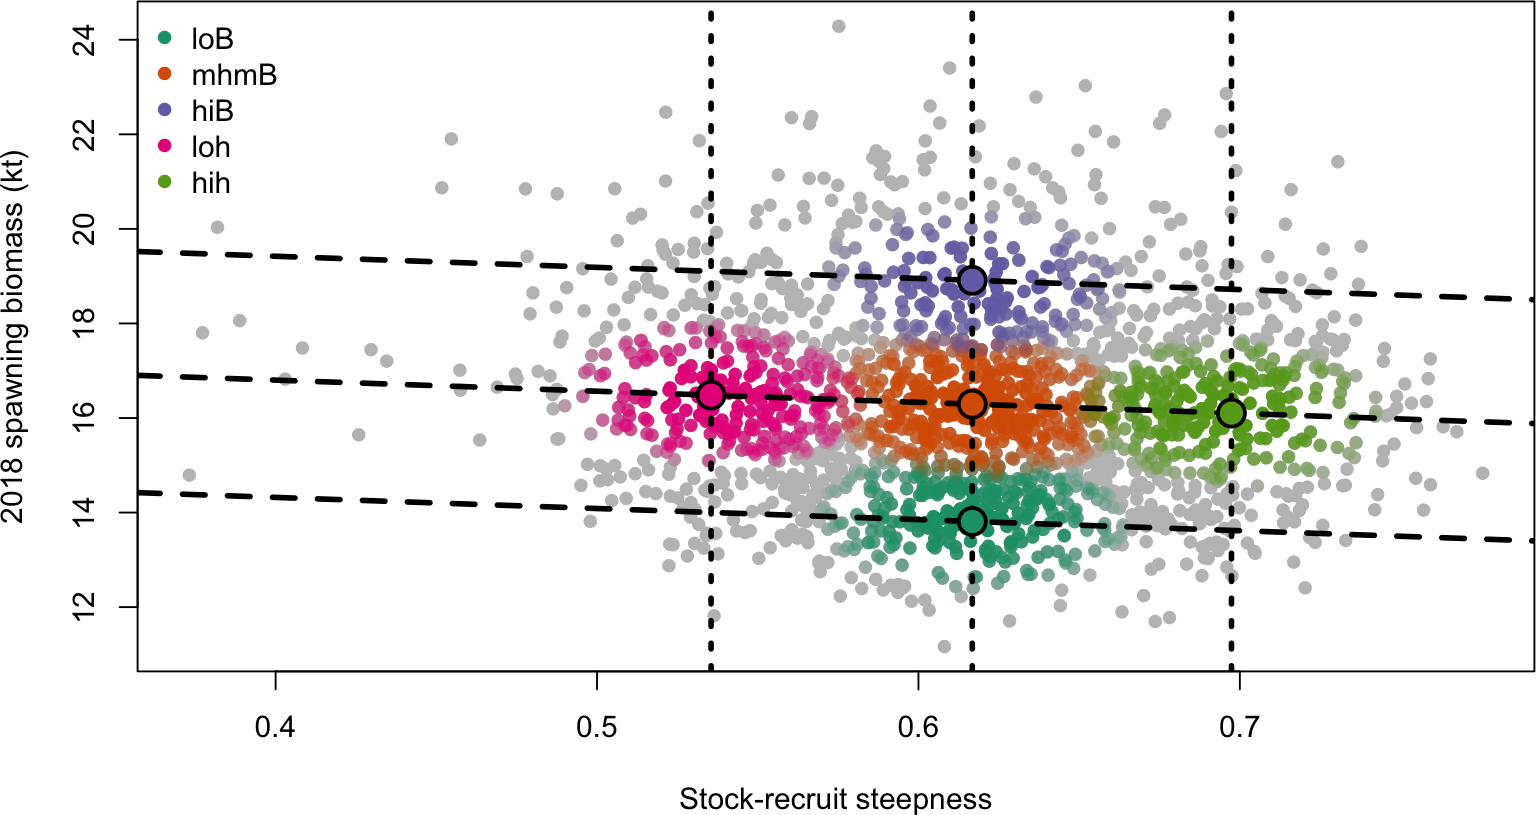
\includegraphics[width=0.9\linewidth]{knitr-figs-pdfunnamed-chunk-17-1}}{Figure \ref{fig:unnamed-chunk-17}} 

}

\caption{Joint marginal posterior distribution MCMC samples (grey dots) for stock-recruit steepness ($h$; $x$-axis) and spawning biomass in 2018 ($B_{2018}$; $y$-axis). Dashed lines indicate the mean, 10th and 90th percentiles of each marginal distribution, with the percentiles of the spawning biomass distribution adjusted to match the regression line between the two marginal distributions. Coloured dots with black borders at the intersections of selected percentiles are the sample centres for the 5 productivity and biomass operating model scenarios with labels matching columns of Table 1, with the coloured posterior MCMC samples showing the set of all points within a Mahalanobis distance of .6 from the centre of the same colour.}\label{fig:unnamed-chunk-17}
\end{figure}
\begin{figure}[htb]

{\centering \pdftooltip{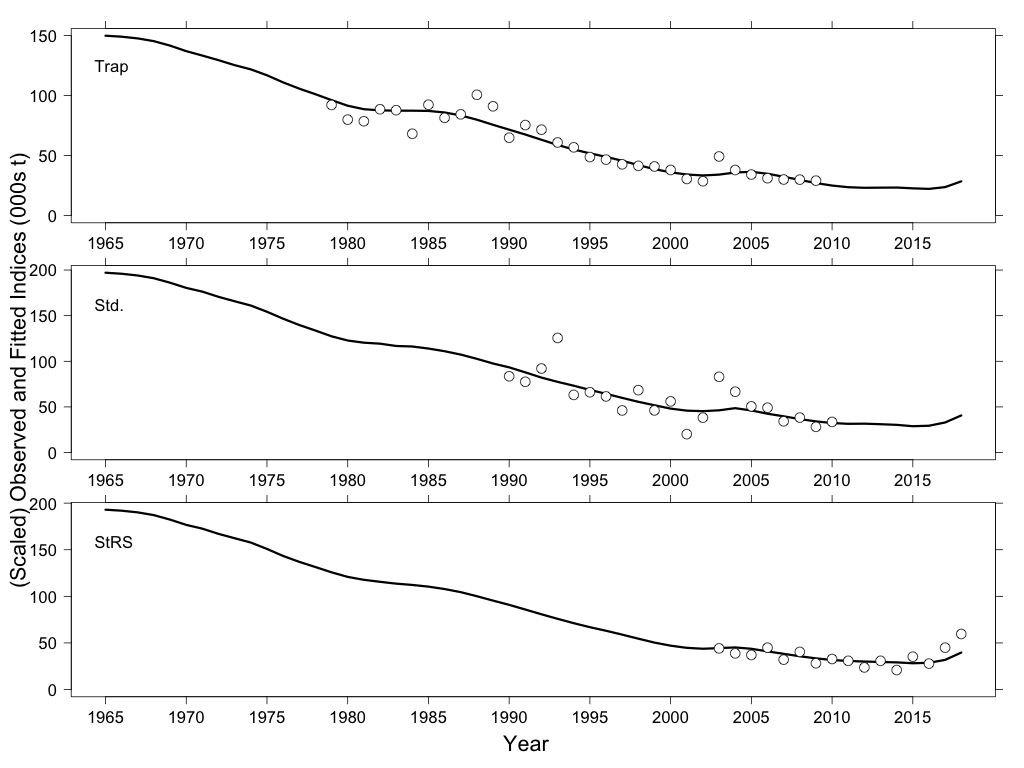
\includegraphics[width=0.9\linewidth]{data/base_ALK_mUnsexed/plotMLEindices}}{Figure \ref{fig:unnamed-chunk-19}} 

}

\caption{Operating model fits to Catch per Unit of Effort (CPUE) indices (kg/trap) from the commercial trap fishery (Trap, top), standardized Sablefish survey (Std., middle), and stratified random Sablefish survey (StRS, bottom). Points show observations scaled by catchability, and lines show operating model vulnerable biomass.}\label{fig:unnamed-chunk-19}
\end{figure}
\newpage
\begin{figure}[htb]

{\centering \pdftooltip{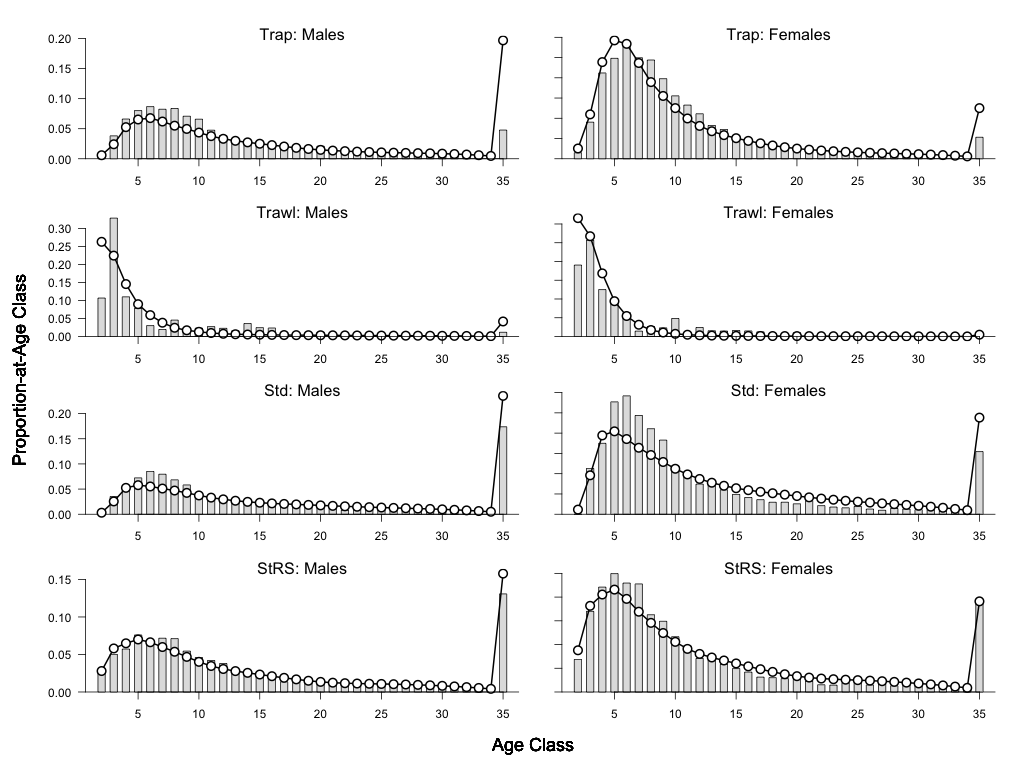
\includegraphics[width=0.9\linewidth]{data/base_ALK_mUnsexed/plotFitAgeFreq_avg}}{Figure \ref{fig:unnamed-chunk-20}} 

}

\caption{Averaged operating model fits to age observations for, from top to bottom, the commercial trap fishery (Trap), commercial trawl fishery (Trawl), standardized survey (Std.), and stratified random survey (StRS). Grey bars are the average proportion of age observations, and the points joined with a line show the average expected distribution of age observations in the operating model. Averages are taken over the years with observations.}\label{fig:unnamed-chunk-20}
\end{figure}
\newpage

\newpage
\begin{turn}

\begin{figure}[htb]

{\centering \pdftooltip{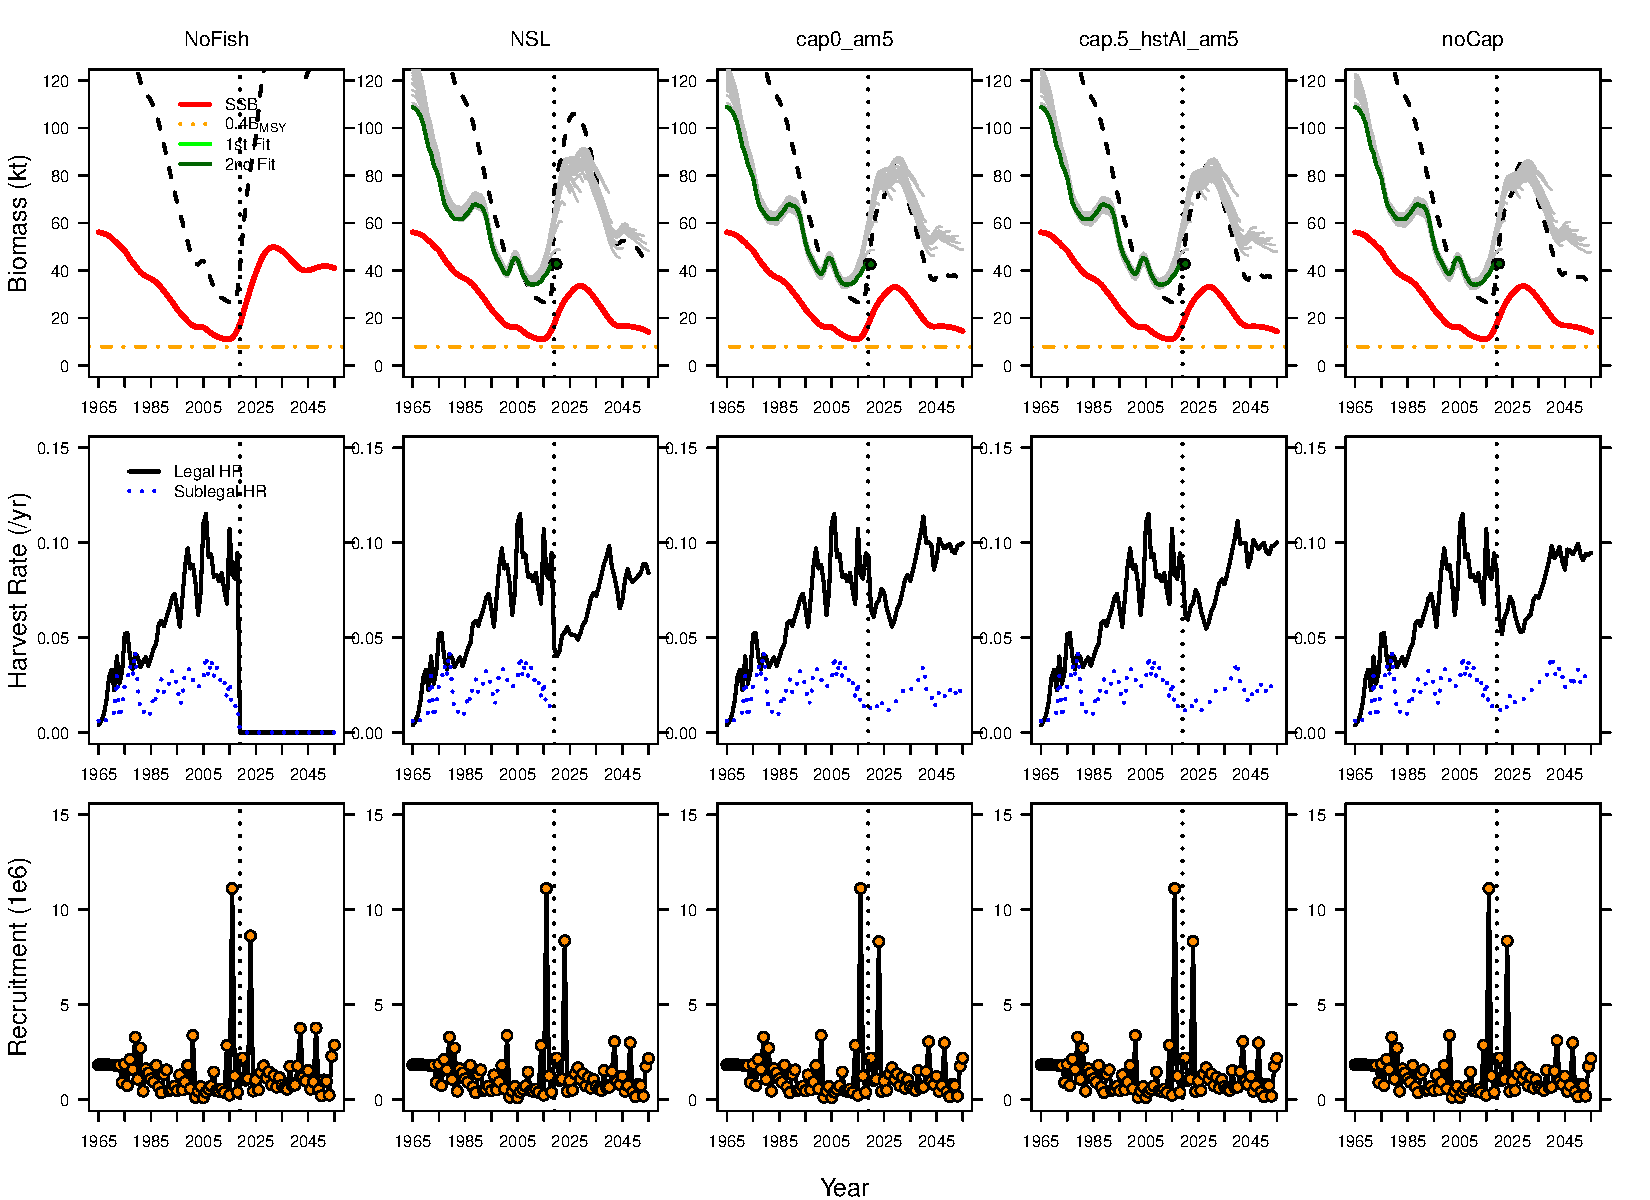
\includegraphics[width=0.8\linewidth]{data/BtFitUtRt/hiRec2016_wtd/hstAl_am5/BtFitUtRt_rep13}}{Figure \ref{fig:unnamed-chunk-22}} 

}

\caption{A single simulation replicate drawn from the \textbf{reference operating models} with the high estimated 2015 year class. The top row of panels show the spawning biomass (red line), legal biomass (black dashed line), and surplus production model estimated biomass (green and grey lines) when estimated as part of the management procedure. The middle row shows the legal (black solid line) and sub-legal (blue dotted line) harvest rates, and the bottom row shows the OM recruitments (black line with orange points). First and second fit refer to the first and second years that the management procedure was applied.}\label{fig:unnamed-chunk-22}
\end{figure}
\newpage


\begin{figure}[htb]

{\centering \pdftooltip{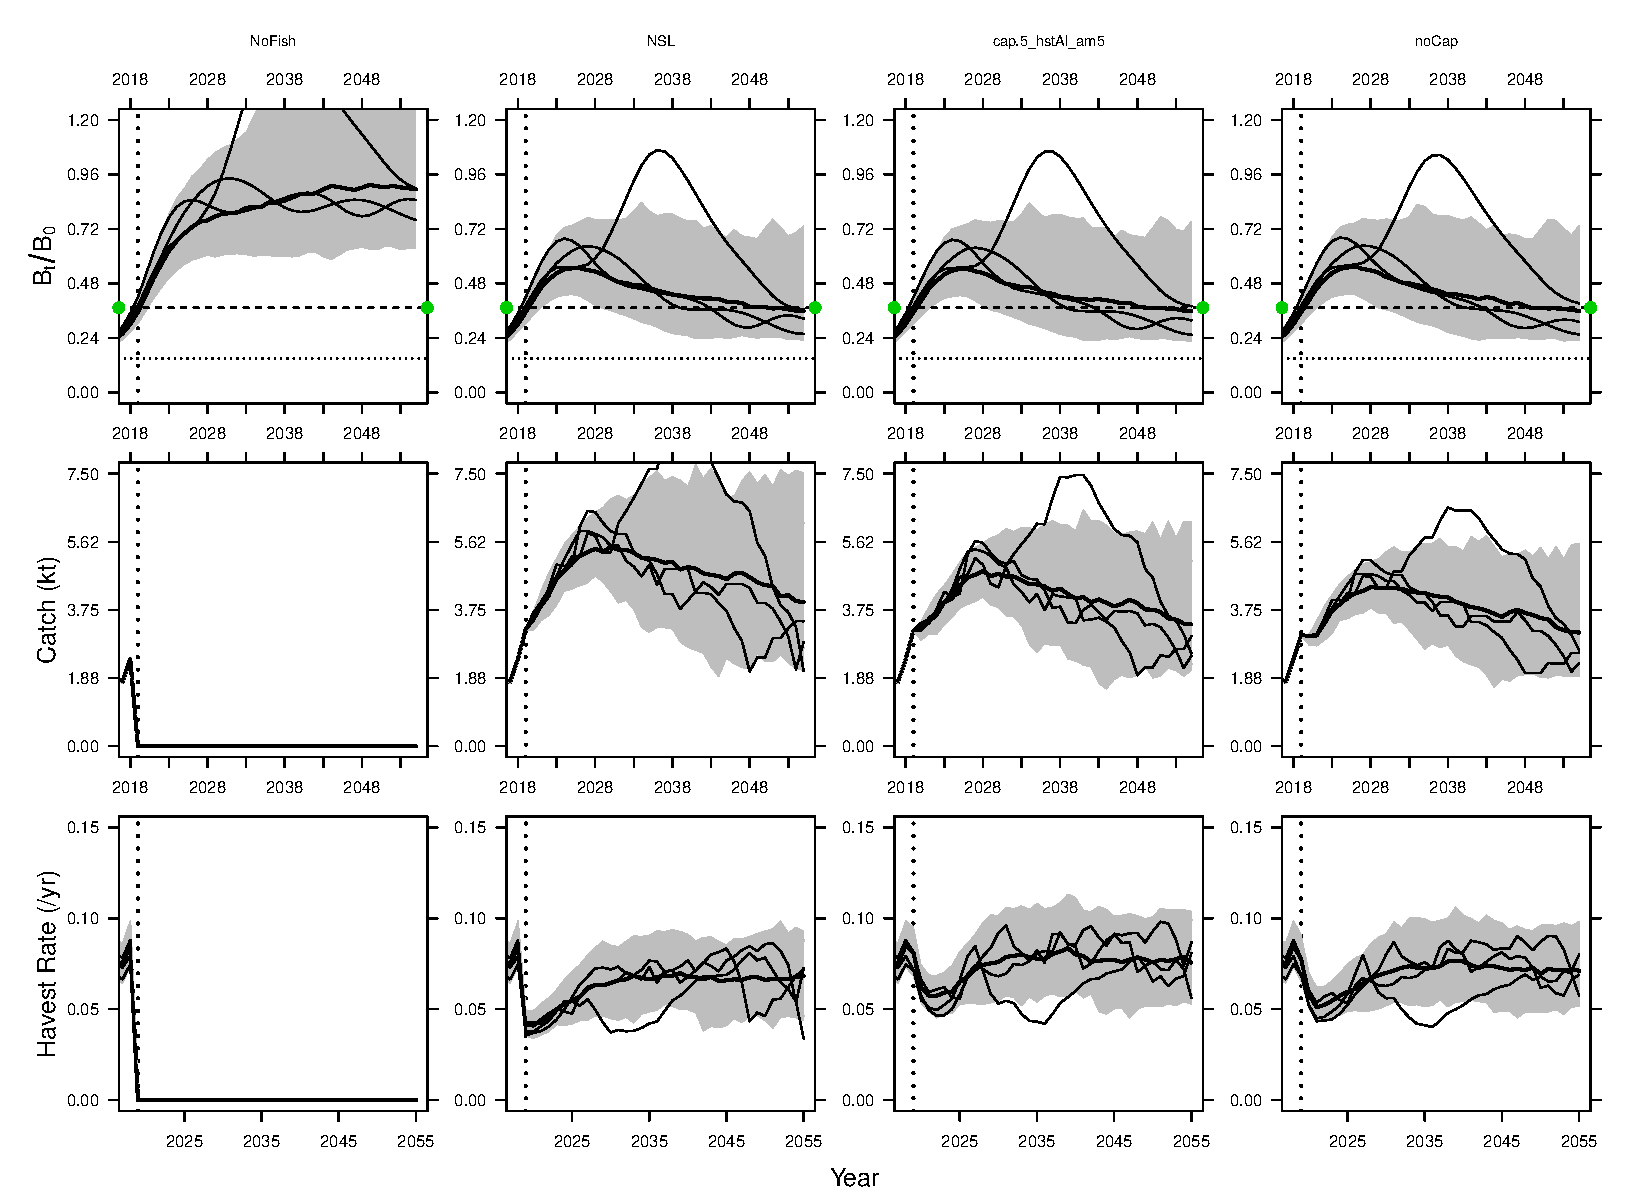
\includegraphics[width=0.8\linewidth]{data/tulipPlots/hiRec2016_wtd/depCatchHR/hiRec2016_wtd_depCatchHR_hstAl_am5}}{Figure \ref{fig:unnamed-chunk-24}} 

}

\caption{Weighted combined simulation envelopes from the 5 productivity and biomass operating models in the \textbf{reference recruitment scenario}, showing the current MP (noCap),three illustrative at-sea-release regulation MPs, and the no fishing MP (NoFish). The top row shows projected biomass relative to unfished, the second row shows the landed catch, and the bottom row shows the legal harvest rate. In each panel, median projections are shown as thick black lines, the central 90 \% of the envelope is shown as grey shading, and the three illustrated simulation replicates as thin black lines. In the top row the green line is $B_{MSY}$ and the lower dashed line is the Limit Reference Point (0.4$B_{MSY}$).}\label{fig:unnamed-chunk-24}
\end{figure}
\newpage
\begin{figure}[htb]

{\centering \pdftooltip{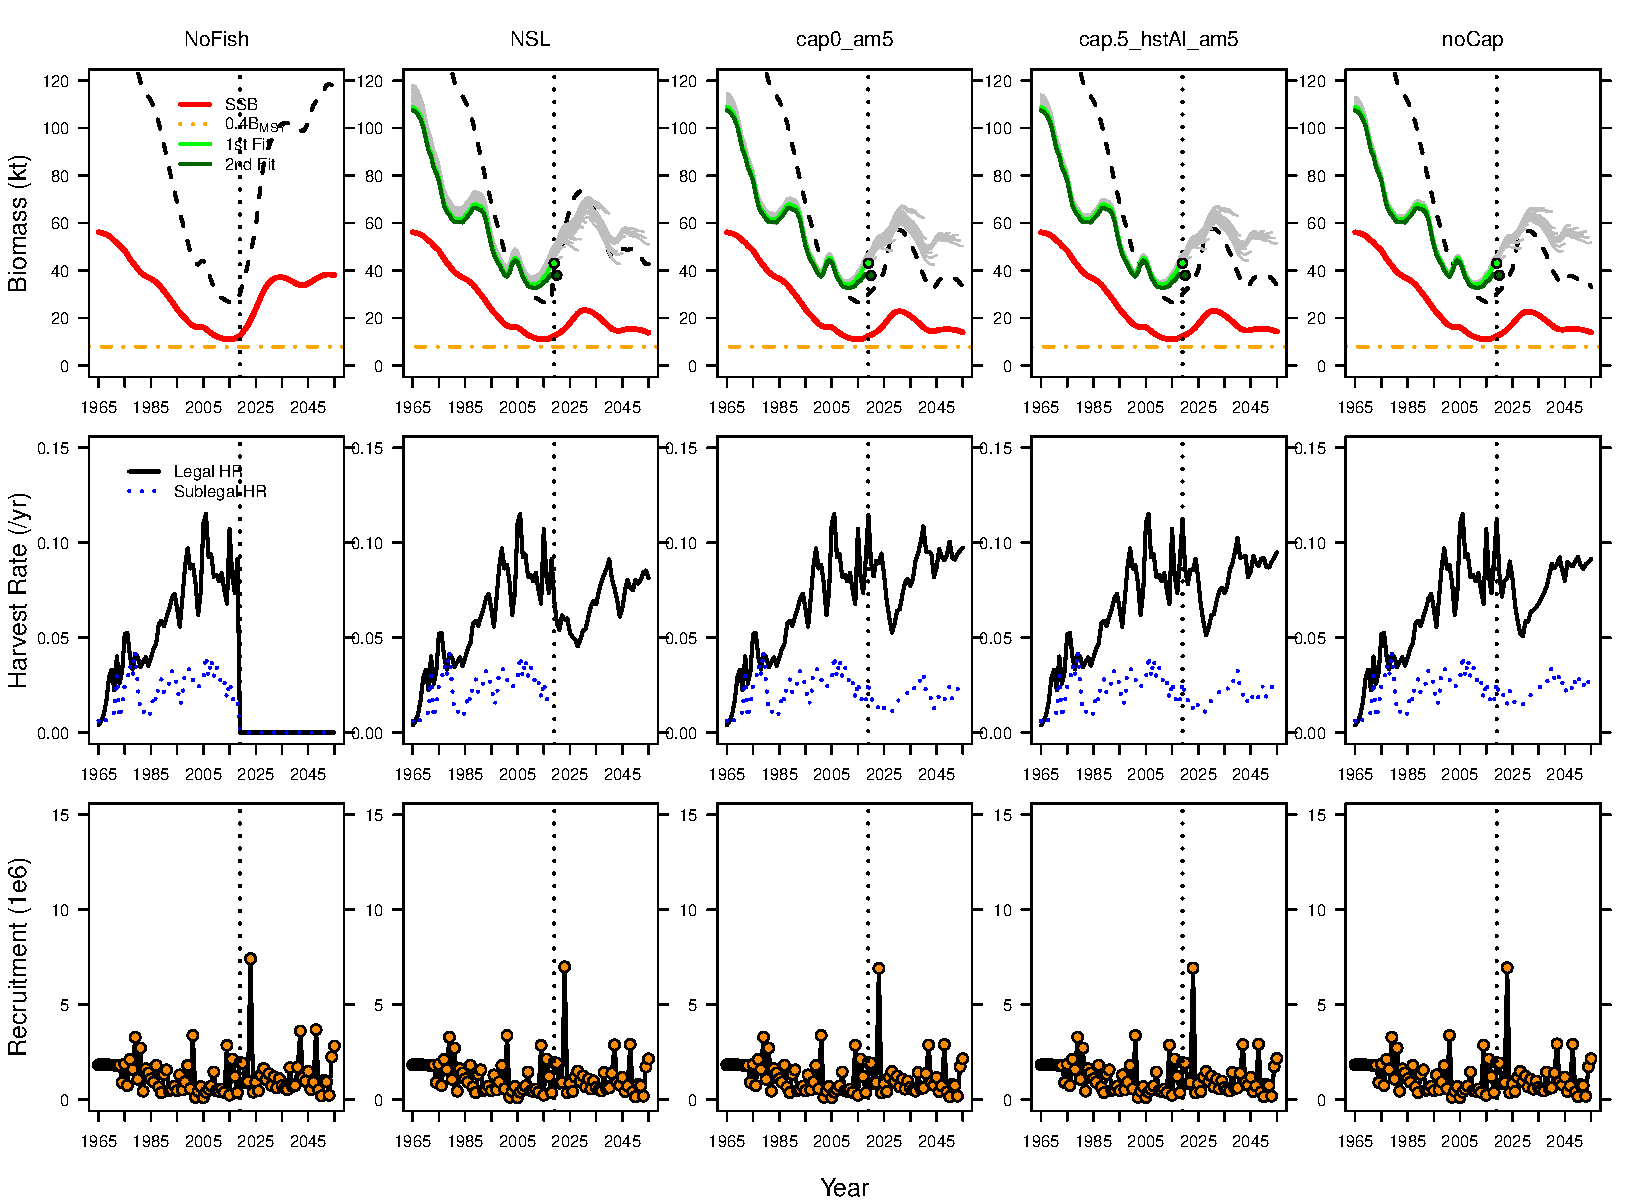
\includegraphics[width=0.8\linewidth]{data/BtFitUtRt/simRec2016_wtd/hstAl_am5/BtFitUtRt_rep13}}{Figure \ref{fig:unnamed-chunk-25}} 

}

\caption{A single simulation replicate drawn from the \textbf{robustness operating models} with a stochastically simulated 2015 year class. The top row of panels show the spawning biomass (red line), legal biomass (black dashed line), and surplus production model estimated biomass (green and grey lines) when estimated as part of the management procedure. The middle row shows the legal (black solid line) and sub-legal (blue dotted line) harvest rates, and the bottom row shows the OM recruitments (black line with orange points). First and second fit refer to the first and second years that the management procedure was applied.}\label{fig:unnamed-chunk-25}
\end{figure}

\newpage
\begin{figure}[htb]

{\centering \pdftooltip{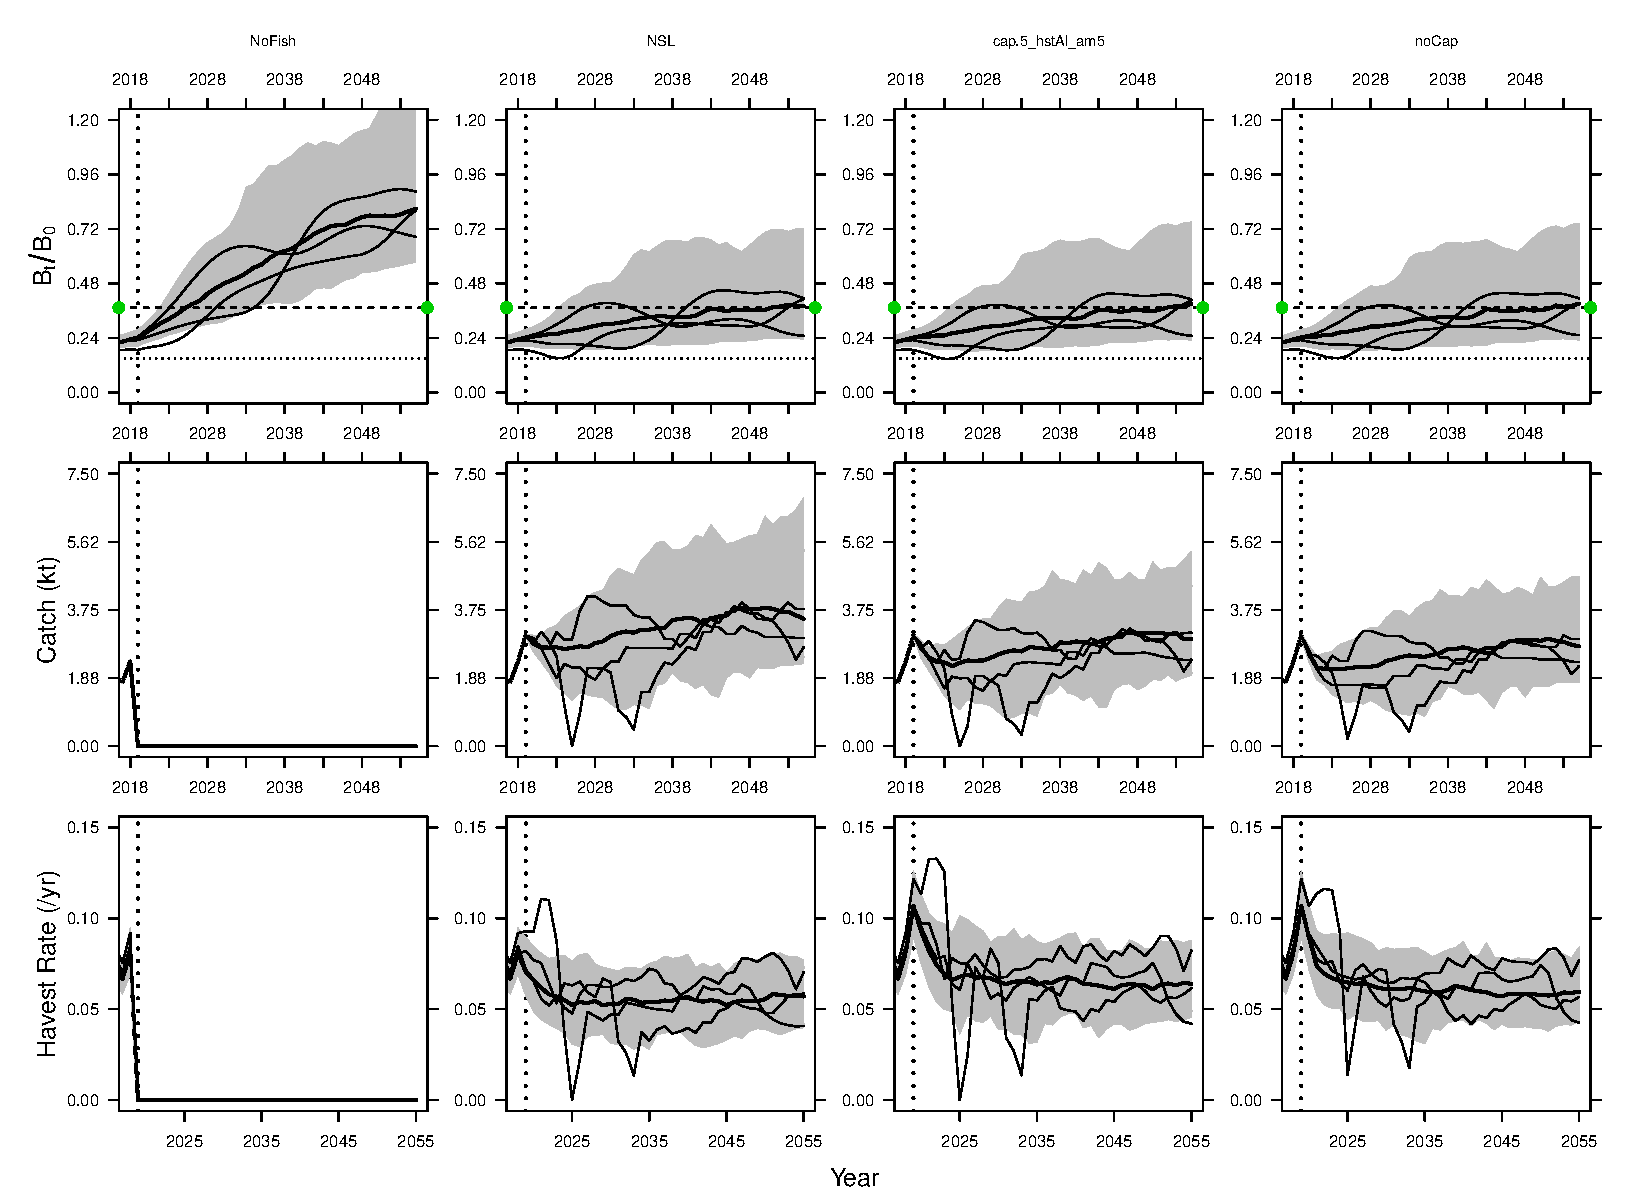
\includegraphics[width=0.8\linewidth]{data/tulipPlots/simRec2016_wtd/depCatchHR/simRec2016_wtd_depCatchHR_hstAl_am5}}{Figure \ref{fig:unnamed-chunk-26}} 

}

\caption{Weighted combined simulation envelopes from the 5 productivity and biomass operating models in the \textbf{robustness recruitment scenario}, showing the current MP (noCap), three illustrative at-sea-release regulation MPs, and the no fishing MP (NoFish). The top row shows projected biomass relative to unfished, the second row shows the landed catch, and the bottom row shows the legal harvest rate. In each panel, median projections are shown as thick black lines, the central 90 \% of the envelope is shown as grey shading, and the three illustrated simulation replicates as thin black lines.In the top row the green line is $B_{MSY}$ and the lower dashed line is the Limit Reference Point (0.4$B_{MSY}$).}\label{fig:unnamed-chunk-26}
\end{figure}
\end{turn}
\hypertarget{appendix}{%
\section{\texorpdfstring{Appendix\label{sec:app-minor}}{Appendix}}\label{appendix}}

\hypertarget{updated-ageing-error-matrix}{%
\subsection{Updated ageing error matrix}\label{updated-ageing-error-matrix}}

The Sablefish age-structured assessment model relies on catch-at-age data to estimate the true age-composition of the population; however, observed catch-at-age data are based on otolith readings that are imperfectly known. Failure to account for errors in otolith readings may lead to smoothing estimates of age-classes, making it more difficult to detect strong recruitment years or stock-recruit relationships (Hanselman et al. \protect\hyperlink{ref-hanselman2012statistical}{2012}). Ageing errors may also bias estimates of growth parameters, maturity schedules, and natural mortality that can lead to overfishing or inaccurate yield projections (Lai and Gunderson \protect\hyperlink{ref-lai1987effects}{1987}; Tyler et al. \protect\hyperlink{ref-tyler1989implications}{1989})

To account for ageing-error, the Sablefish age-structured operating model uses an ageing error matrix. In this MSE cycle, we simplified the formulation of the ageing-error matrix from the previously used double-geometric model to a discretized normal distribution. The two major differences between these two formulations are (i) that the error structure is constrained to be symmetric for the normal formulation, while the double geometric model allows for some skew in the error distribution; and (ii) the normal assumes the assigned true age is the mode of the normal density, forcing ageing errors to be on average unbiased.

We developed our ageing error matrix using otoliths that had been read by two different readers at the DFO Pacific Biological Station ageing lab. These data account for approximately 15\% of the total otolith readings for BC Sablefish, which are read first by the primary reader and then by a secondary reader as a quality control. In the majority of cases both readers agreed (62\%) and in cases where the two readings differ (38\%), both readers conferred to resolve the discrepancy and agree on the final age assigned (Pers. Comm, J. Groot, DFO). In most cases the final age reading was that assigned by the secondary or primary reader (36\%), but in a few cases a new age was assigned (2\%).

We applied statistical models for estimating the probability of observing an age class (a) given the true age (b) based on methods described in Richards et al. (\protect\hyperlink{ref-richards1992statistical}{1992}) and Heifetz et al. (\protect\hyperlink{ref-heifetz1999age}{1999}). The model assumes a normal ageing-error distribution where the estimated standard deviation of the observed age for a true age b is based on three parameters \(\Phi = \{ \sigma_1, \sigma_A, \alpha \}\) in the form:
\begin{equation}
\sigma(b) = \left\{
    \begin{array}{ll}
        \sigma_1 + (\sigma_A - \sigma_1) \frac{1 - e^{-\alpha(b - 1)} }{1 - e^{-\alpha(A - 1)}}, & \alpha \neq 0; \\
        \sigma_1 + (\sigma_A - \sigma_1) \frac{b-1}{A-1}, & \alpha = 0.\\
    \end{array} \right.
\end{equation}
Parameters \(\sigma_1\) and \(\sigma_A\) are the standard deviations for \(b=1\) and \(b=A\), representing the minimum and maximum ages, respectively. The \(\alpha\) parameter determines the non-linearity of the function, such that\textasciitilde{}\(\sigma(b)\) becomes linear as \(\alpha \rightarrow 0\). The age-error matrix is defined as:
\begin{align}
q(a \vert b, \Phi) &= \frac{x_{ab}(\Phi)}{\sum_{a = 1}^A x_{ab}(\Phi) }; \\
x_{ab} &= \frac{1}{\sqrt{2\pi}\sigma(b)} e^{-\frac12 \left[ \frac{a-b}{\sigma(b)} \right]^2}.
\end{align}
Given that the true age of the fish is unknown, it is not possible to accurately determine bias in the age readings and whether certain age classes are more likely to be under or over-estimated. We tested 2 different approaches for the assumed ``true age'', using 1) the mean of the two reader ages rounded to the nearest integer (Heifetz et al. \protect\hyperlink{ref-heifetz1999age}{1999}), and 2) the final age assigned. For both approaches we set \(A=90\), based on the maximum assigned age by the readers.

The likelihood \(\mathcal{L}\) of observed ages \(A\) given true ages B is then defined as:
\begin{equation}
\mathcal{L}(A \vert B) = \prod_{i = 1}^I \prod_{j = 1}^J q(a_{ij} \vert b_i \Phi),
\end{equation}
where \(b_i\) is the assumed `true age' of fish \(i\), and \(a_{ij}\) is the age assigned by reader \(j\) to the individual fish \(i\). Maximum likelihood parameter estimates, predicted standard deviation at age, and age-error matrices are provided below (Table 9, Figures 8-9)

\hypertarget{trawl-age-length-key-and-updated-selectivity-curve}{%
\subsection{Trawl Age-Length Key and updated selectivity curve}\label{trawl-age-length-key-and-updated-selectivity-curve}}

The Sablefish age-structured operating model uses observations of catch at age from commercial fisheries to estimate natural mortality and gear selectivity functions. Trawl selectivity has been identified a key determinant in reducing uncertainty in estimates of sub-legal Sablefish catch and releases (Cox et al. \protect\hyperlink{ref-cox2019evaluating}{2019}), as up until now the trawl selectivity model was heavily dependent on priors for a normal selectivity curve estimated from tagged fish recovered (within one year from release) in the commercial trawl fishery. To improve estimates of legal and sub-legal fishing mortality from the trawl sector, we leveraged catch-at-age and catch-at-length data from BC trawl fisheries to develop a sex-specific age-length key, which was in turn used to increase the catch-at-age sample size.

To develop our age-length key, we used all available catch-at-age data collected from observed trips in the commercial trawl fishery. We then used this to populate an empirical age-length frequency matrix, binning fish into 3cm length bins and 1 year age classes. We defined this matrix as \begin{equation}
F = \left[ n_{l,a} \right],
\end{equation} where \(n_{l,a}\) is the number of fish observed in length bin \(l\) and age class \(a\). The matrix \(A\) was converted to a probability of age-at-length \(l\) matrix \(P\) by normalising the columns of \(A\) \begin{equation}
P_{l,a} = F_{l,a} / \sum_{a'} F_{l,a'}. 
\end{equation}
We then generated expected age composition data by applying the matrix \(P\) to length compositions \(C_l\) derived from the commercial trawl catch-at-length data. \begin{align}
C_a &= P^T \cdot C_l,
\end{align} where \(P\) is transposed so that the length dimension matches the vector \(C_l\). We restricted \(C_l\) to catch-at-length data from years where at least 5 trips were sampled. We defined keys \(P_m\) and \(P_f\) for male and female fish, respectively, and generated sex-specific age observations (Figures 10-11). Length observations from unsexed fish were treated as male specimens, as the operating model optimisation would not converge when they were treated as females.
Inferred catch-at-age compositions had a noticable effect on the selectivity-at-length curves for the trawl fleet (Figure 12). The fully selected size class moved from about 42 cm to 48 cm, and the shape of the Gamma selection curve dome was narrower, deselecting to about 60\% by the 55cm size limit, as opposed to about 80\% for the normal model in 2016.

\newpage

\clearpage
\begingroup\fontsize{12}{14}\selectfont
\begingroup\fontsize{12}{14}\selectfont
\begin{longtable}[t]{rlrrr}
\caption{\label{tab:unnamed-chunk-28}Ageing error model parameters for both true age cases tested.}\\
\toprule
\textbf{Case} & \textbf{True Age} & \textbf{$\sigma_1$} & \textbf{$\sigma_A$} & \textbf{$\alpha$}\\
\midrule
1 & Mean Reader Age & 0.38 & 4.80 & 0.014\\
2 & Final Age Assigned & 0.89 & 9.35 & -0.008\\
\bottomrule
\end{longtable}
\endgroup{}
\endgroup{}

\clearpage
\begin{figure}[htb]

{\centering \pdftooltip{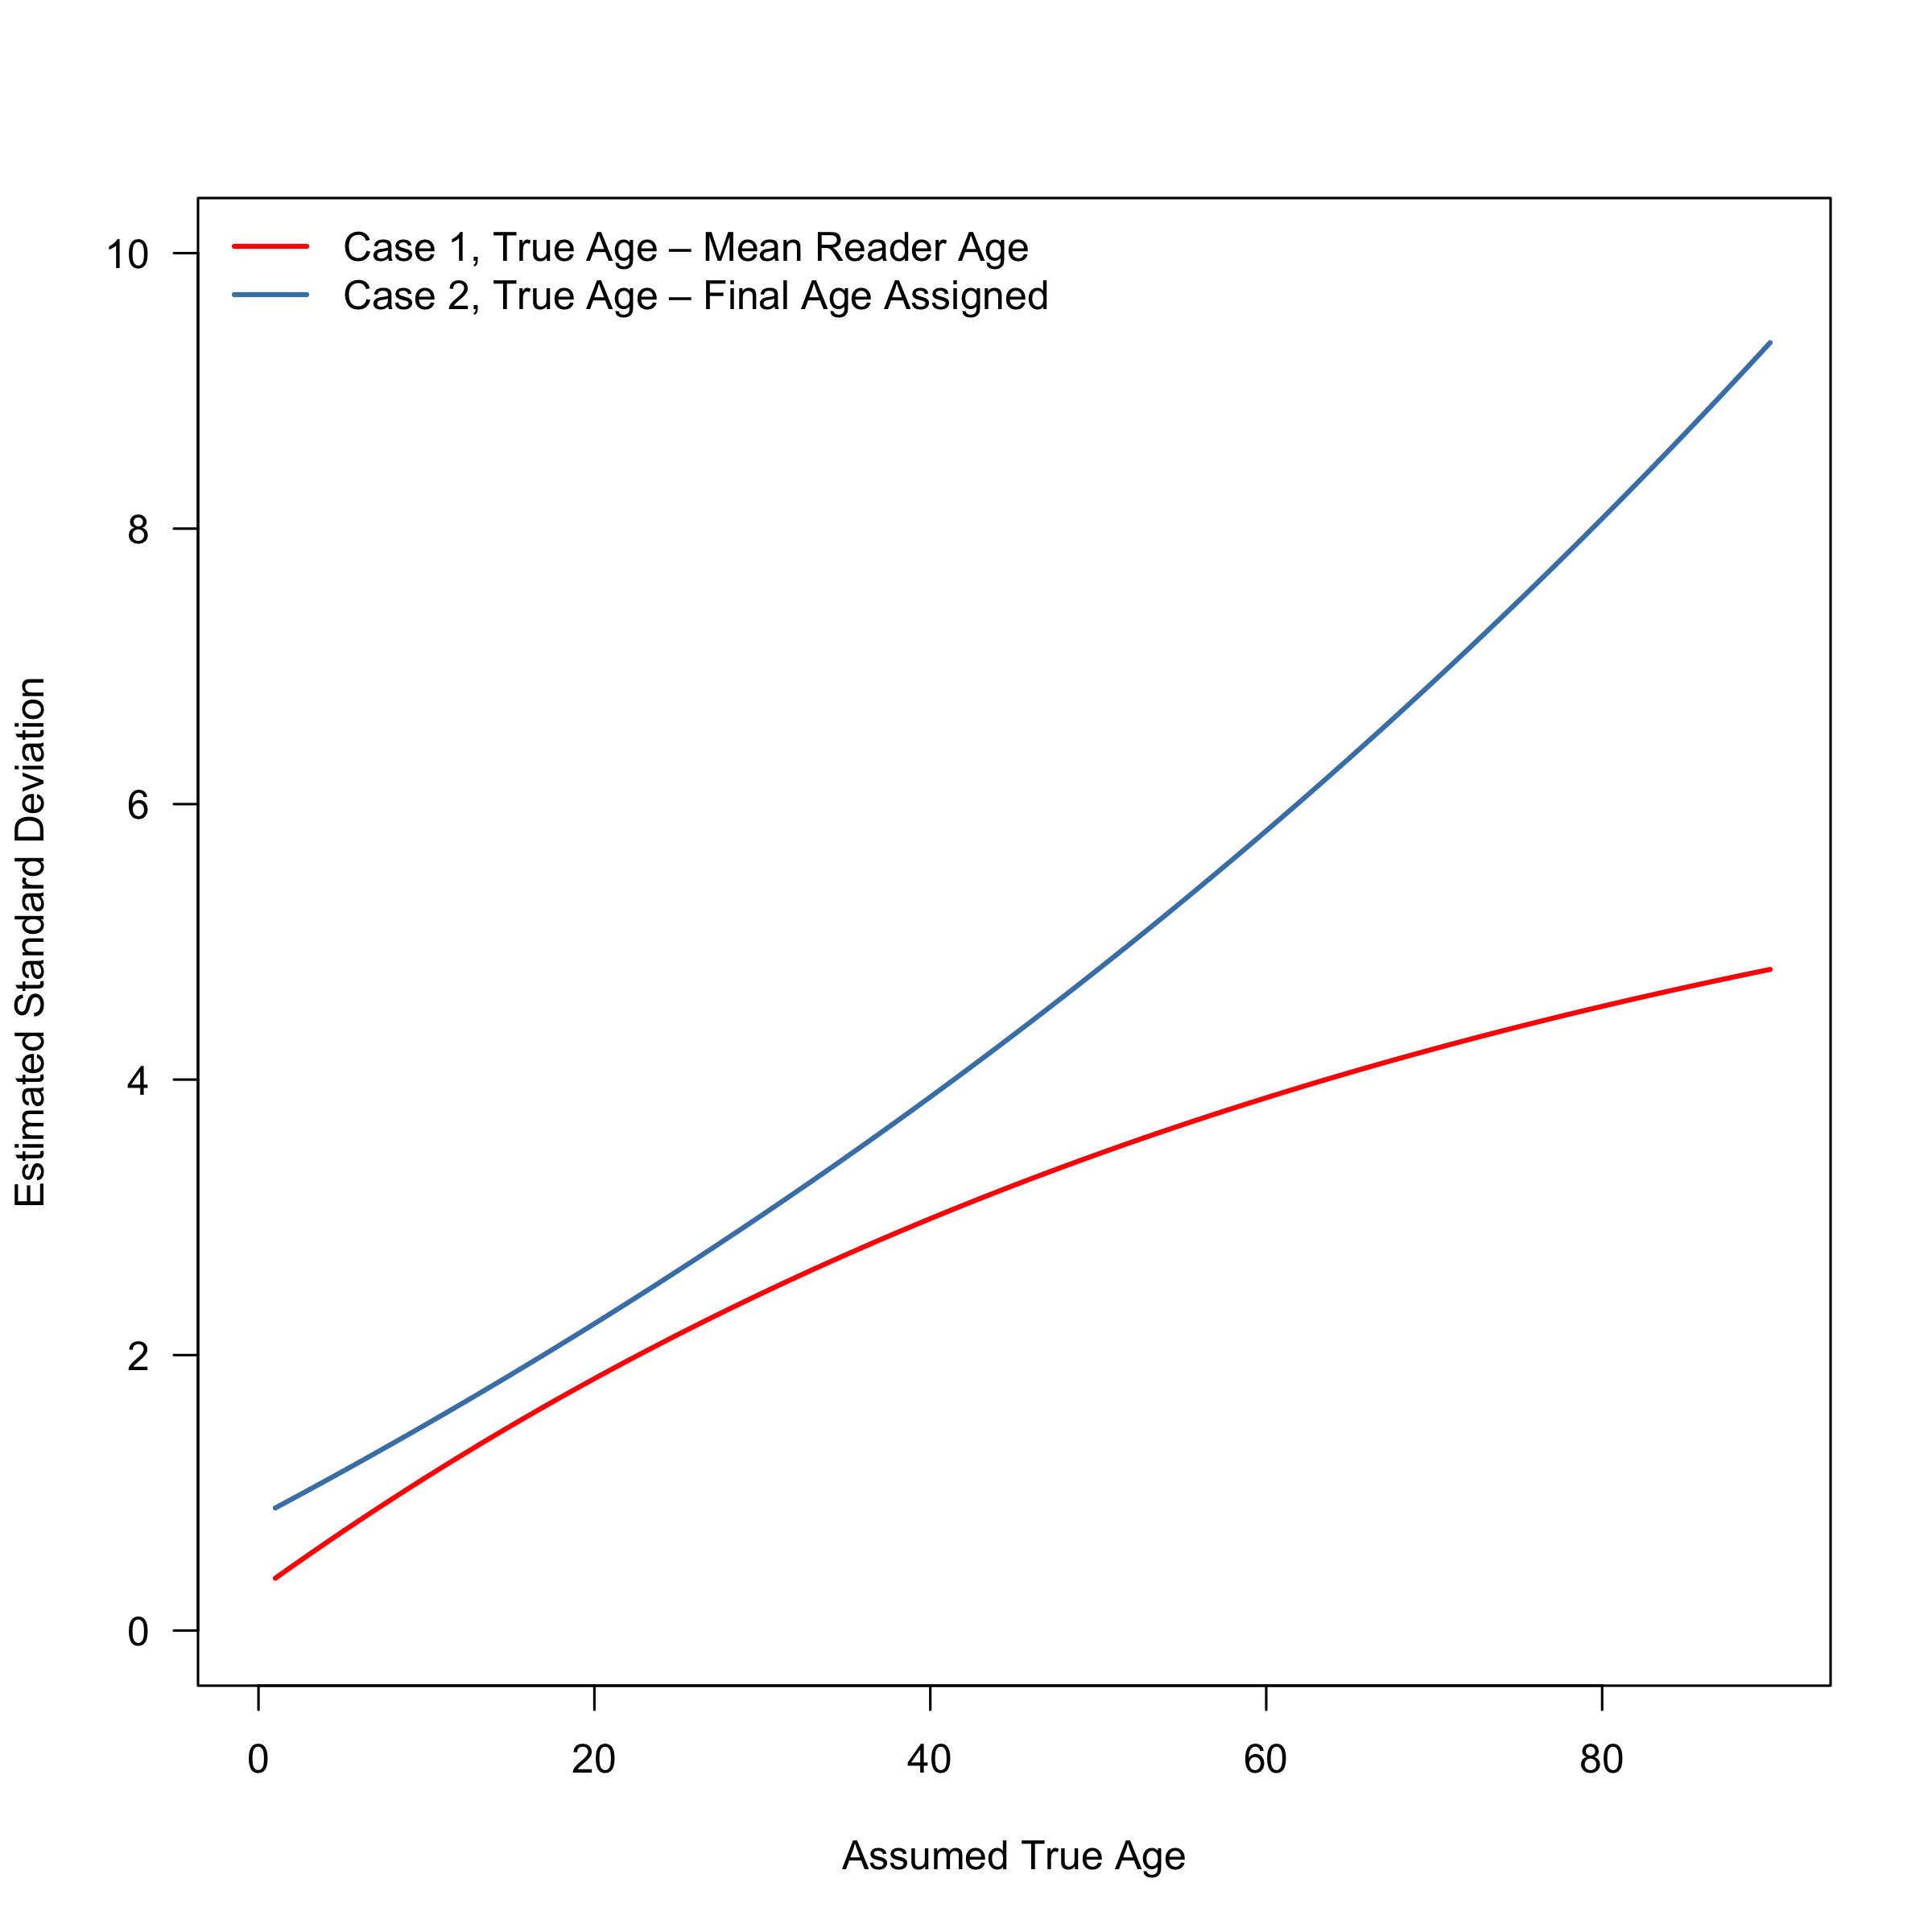
\includegraphics[width=0.9\linewidth]{data/ageErr1}}{Figure \ref{fig:unnamed-chunk-30}} 

}

\caption{Estimated standard deviation of observed ages for the two age assignment cases considered.}\label{fig:unnamed-chunk-30}
\end{figure}
\newpage
\begin{figure}[htb]

{\centering \pdftooltip{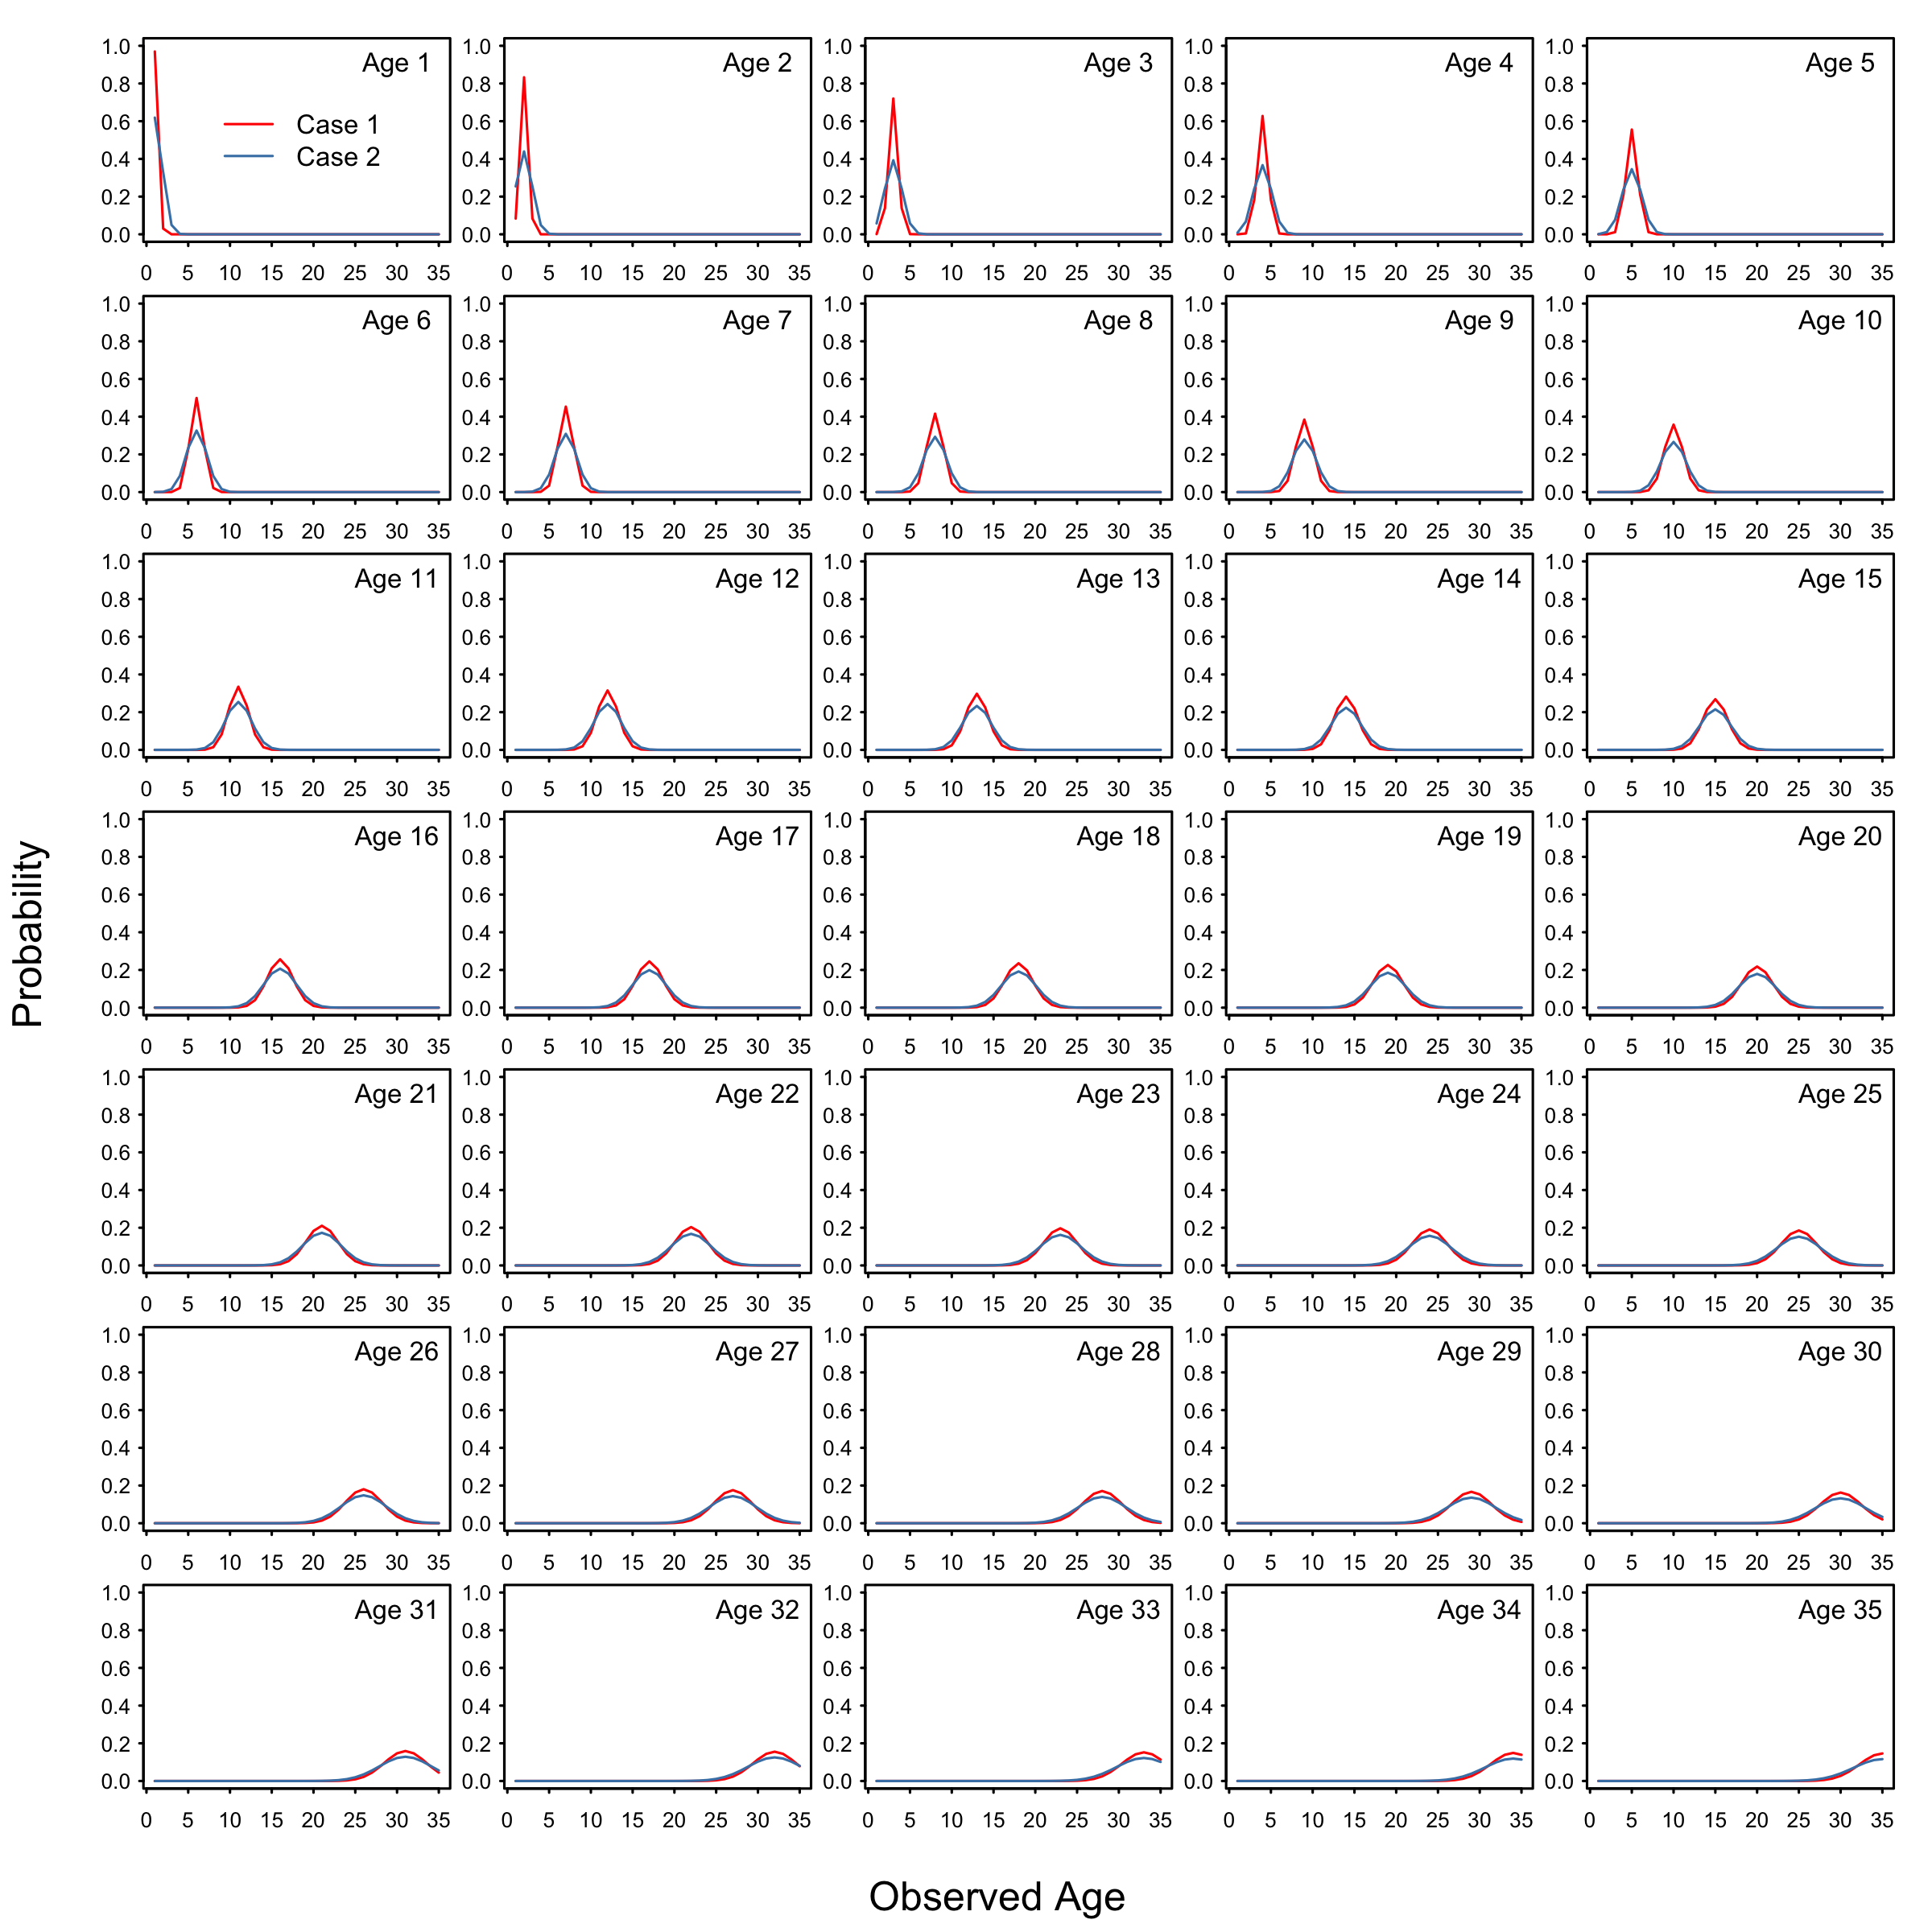
\includegraphics[width=0.9\linewidth]{data/ageErr2}}{Figure \ref{fig:unnamed-chunk-31}} 

}

\caption{Probability of observed ages given the true age indicated in top right corner of each panel for the two age assignment cases considered.}\label{fig:unnamed-chunk-31}
\end{figure}
\newpage
\begin{figure}[htb]

{\centering \pdftooltip{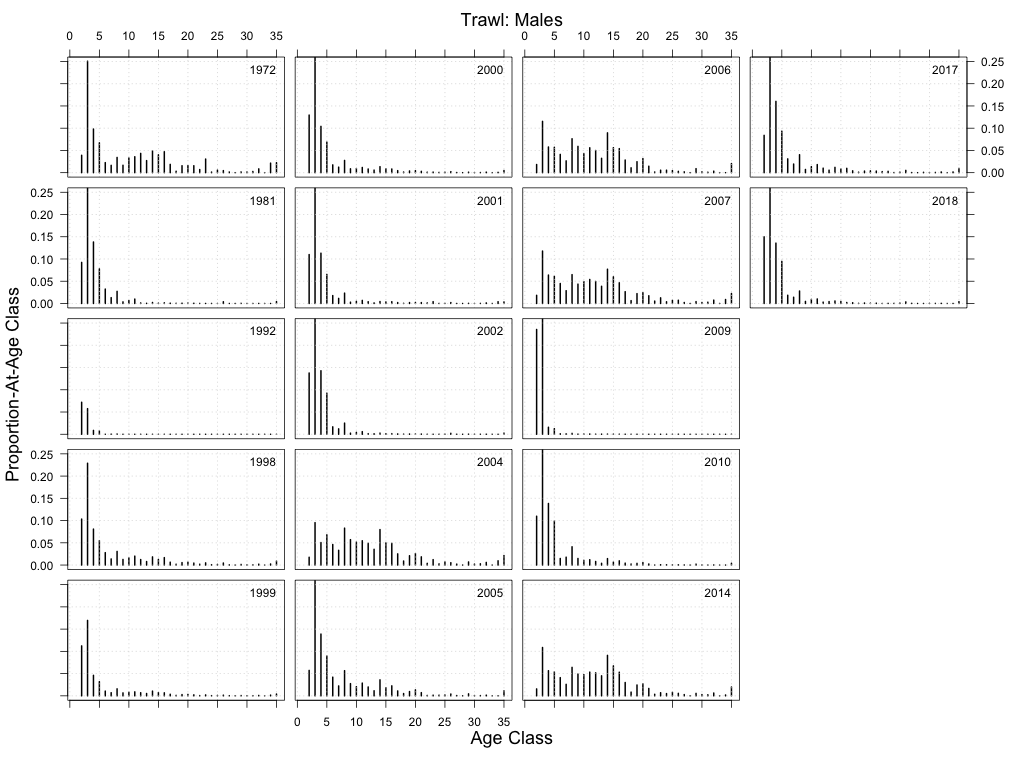
\includegraphics[width=0.9\linewidth]{data/base_ALK_mUnsexed/plotObsAgeFreq_m3}}{Figure \ref{fig:unnamed-chunk-32}} 

}

\caption{Inferred male catch-at-age compositions generated by the trawl age-length key from length observations of male and unsexed fish.}\label{fig:unnamed-chunk-32}
\end{figure}
\newpage
\begin{figure}[htb]

{\centering \pdftooltip{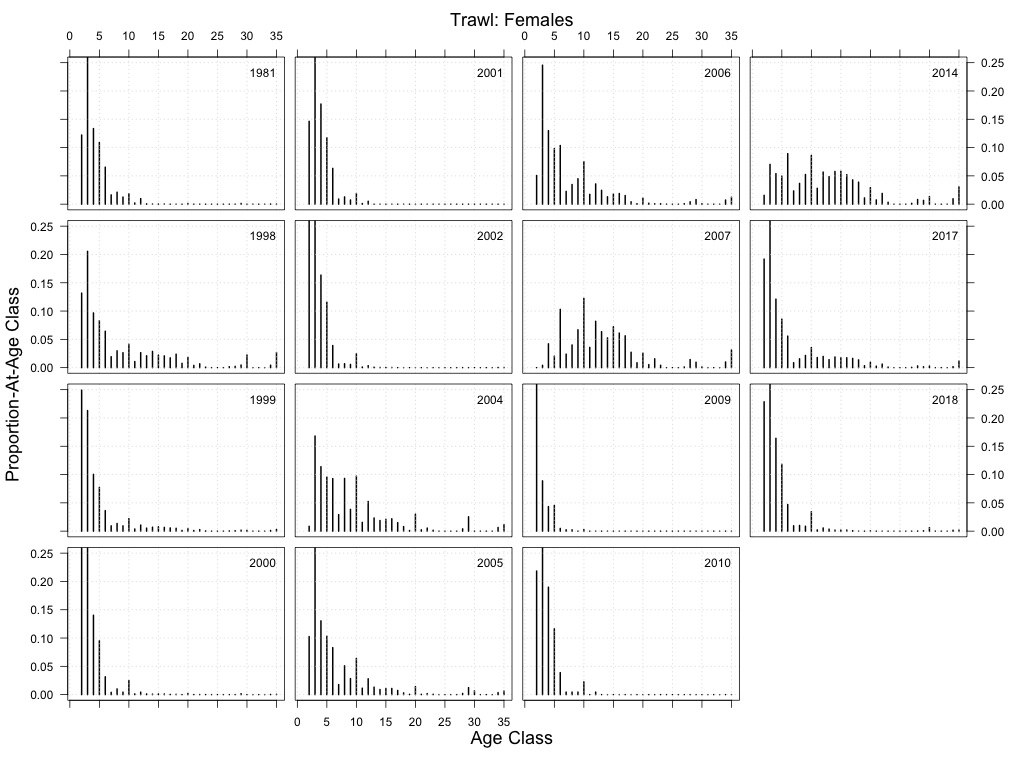
\includegraphics[width=0.9\linewidth]{data/base_ALK_mUnsexed/plotObsAgeFreq_f3}}{Figure \ref{fig:unnamed-chunk-33}} 

}

\caption{Inferred female catch-at-age compositions generated by the trawl age-length key from length observations of female fish}\label{fig:unnamed-chunk-33}
\end{figure}
\newpage
\begin{figure}[htb]

{\centering \pdftooltip{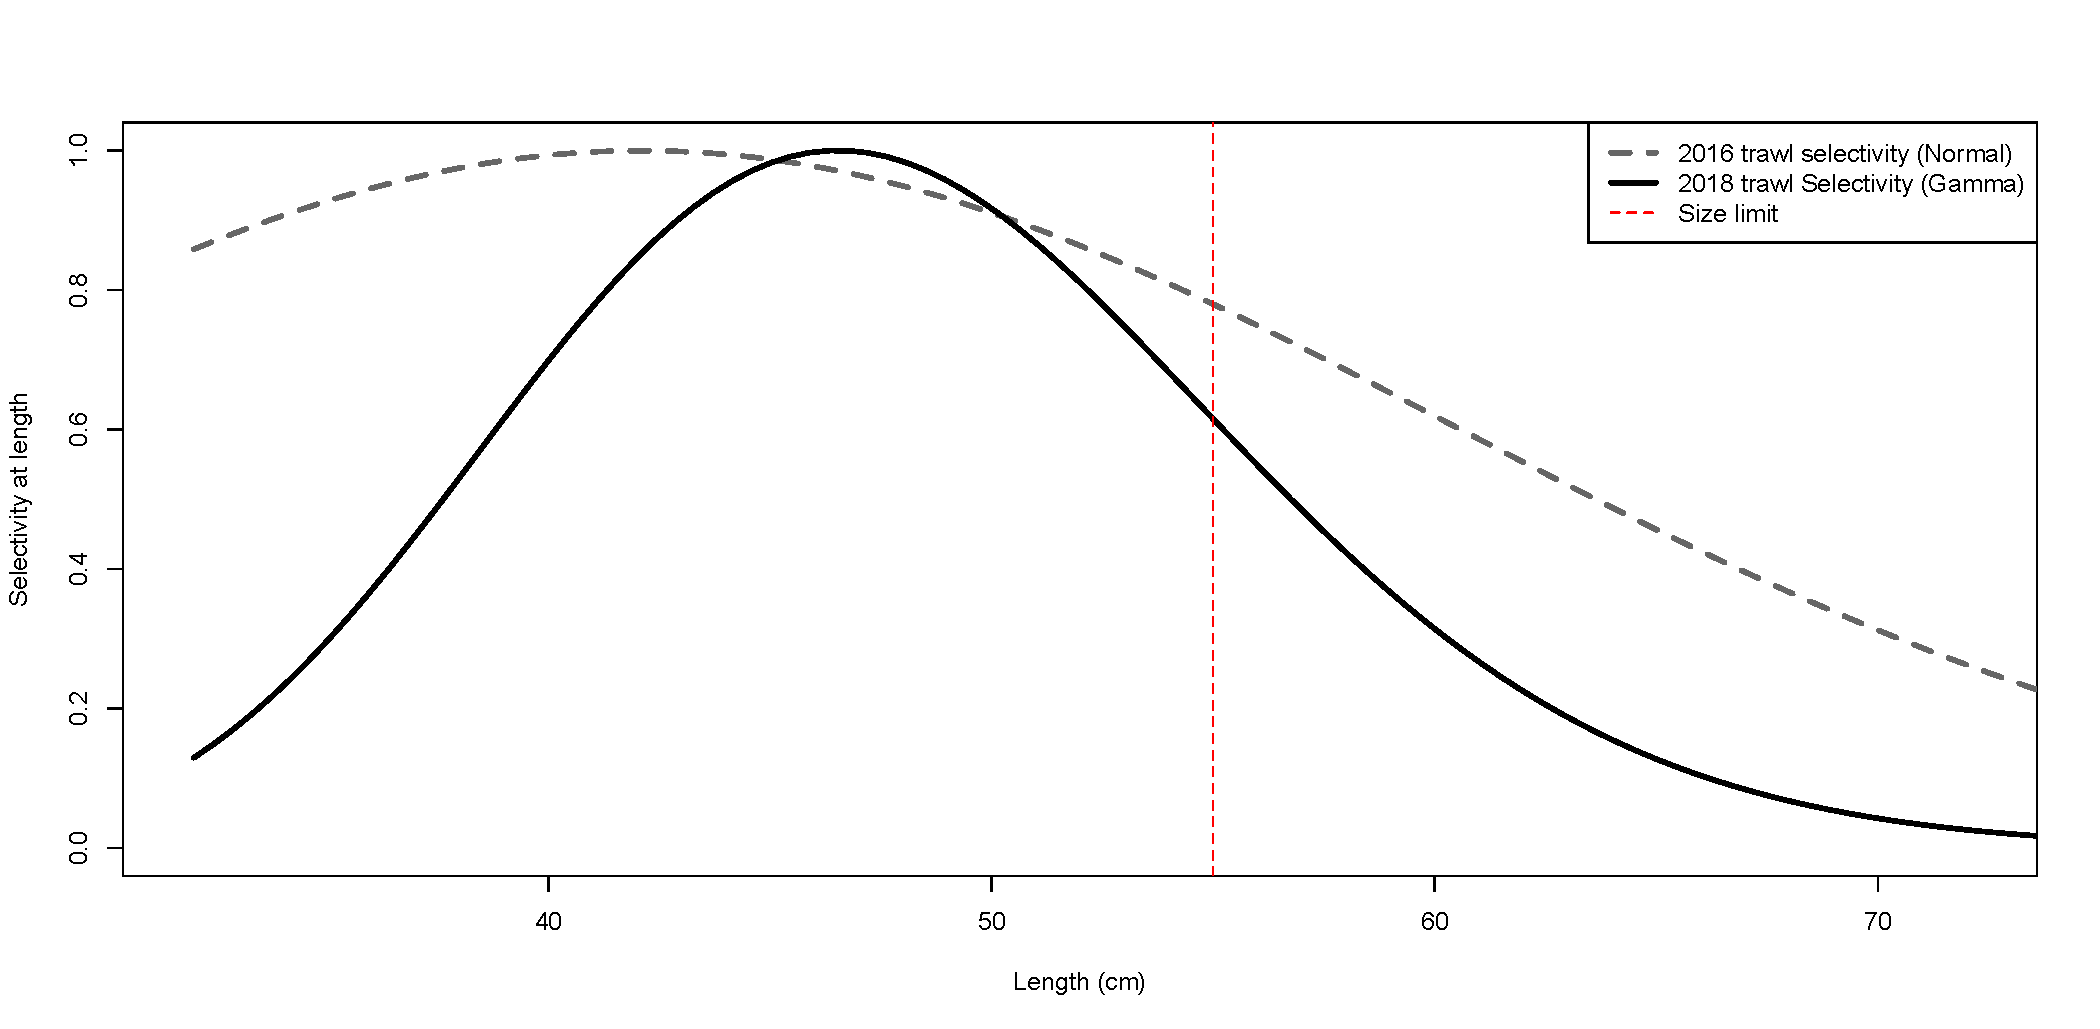
\includegraphics[width=0.9\linewidth]{data/trawlSelOverlay}}{Figure \ref{fig:unnamed-chunk-34}} 

}

\caption{Trawl selectivity-at-length curves from the 2016 operating model (dashed grey line) and 2019 operating model (solid black line), and the legal size limit (vertical red dashed line). The length axis starts at the modeled length at age-1 of 32cm.}\label{fig:unnamed-chunk-34}
\end{figure}
\clearpage

\section{This report is available from the}
\begin{center}
Centre for Science Advice\\
\rdRegion{}\\
Fisheries and Oceans Canada\\
3190 Hammond Bay Rd.\\Nanaimo, BC, V9T 6N7\\
\vspace{0.1cm}
Telephone: (250) 756-7088\\
E-mail: \link{mailto:csap@dfo-mpo.gc.ca}{csap@dfo-mpo.gc.ca}\\
Internet address: \link{http://www.dfo-mpo.gc.ca/csas-sccs/}{www.dfo-mpo.gc.ca/csas-sccs/}\\
\vspace{0.1cm}
ISSN 1919-3769\\
\copyright{} Her Majesty the Queen in Right of Canada, \rdYear{}\\
\vspace{0.2cm}

\includegraphics[scale=0.96]{\locRepo/images/recycle.png}
\end{center}
Correct citation for this publication:

\citeEng{\rdYear{}/\rdNumber{}}

\emph{Aussi disponible en fran\c{c}ais:}

\citeFr{\rdYear{}/\rdNumber{}}

\setlength{\parindent}{0in} \setlength{\leftskip}{0in} \setlength{\parskip}{4pt}
\hypertarget{refs}{}

\end{document}
